%------------------------------------------------------------------------------
\section{Vorbereitung}
%------------------------------------------------------------------------------
In dieser Übung soll das Zusammenspiel grundlegender Internetdienste veranschaulicht werden.
Hierfür werden zwei virtuelle Maschinen benötigt, die im Folgenden erstellt
werden. Die Speicherorte und Bezeichnung können Sie aus der Tabelle
\ref{tab:install-location} entnehmen.
\newline
\newline
\textbf{\textit{Hinweis}}: Die Bezeichnung des Servers erfolgt nach dem
Schema srv\{4.-IP-Octet\}.

\scriptsize
\begin{table}[!h]
  \centering
	\begin{tabular}{l l l l l}
		\hline
		Name & Pfad & Hostname & Benutzername & Passwort \\
		\hline
		srv200 & D:$\backslash$Austausch$\backslash$Internetdienste$\backslash$srv200 &
		srv200 & admin1 & password1 \\
		srv201 & D:$\backslash$Austausch$\backslash$Internetdienste$\backslash$srv201 &
		srv201 & admin2 & password2 \\
		\hline
	\end{tabular}
	\caption{Pfade für die Installation und Einrichtung der virtuellen Maschinen}
	\label{tab:install-location}
\end{table}
\normalsize 

%------------------------------------------------------------------------------
\subsection{Erzeugung der virtuellen Maschinen}
%------------------------------------------------------------------------------
Im Folgenden wird die Erzeugung einer virtuellen Maschine mit VMware-Workstation
exemplarisch für \textbf{srv200} gezeigt. Verfahren Sie für die
Maschine \textbf{srv201} analog. Öffnen Sie das Programm  \textbf{VMware
Workstation} und wählen Sie \textbf{File$\rightarrow$New$\rightarrow$Virtual Machine} im Menü.

\begin{nofloat}{figure}
\begin{center}
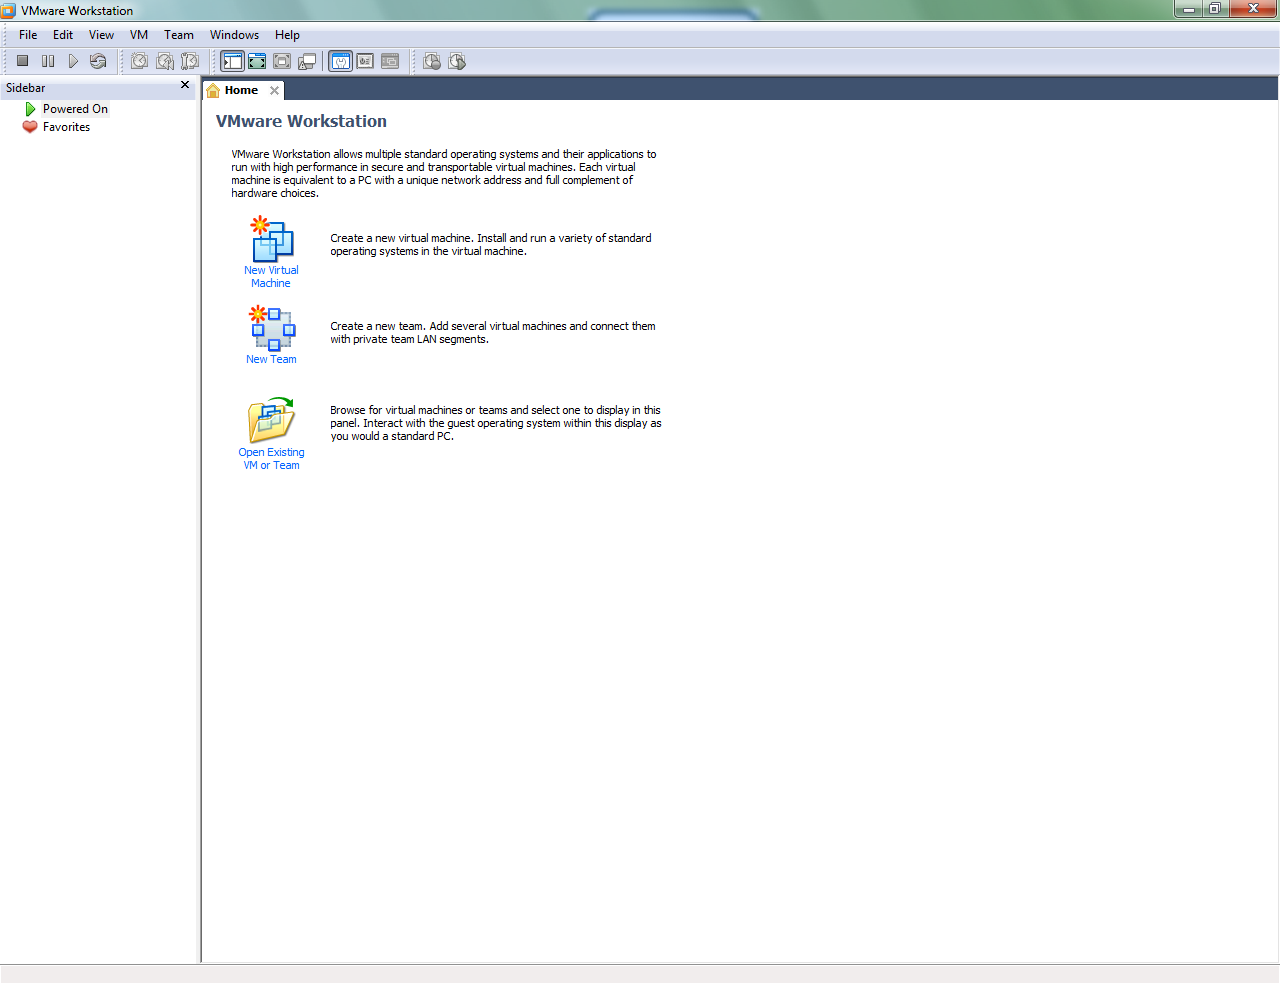
\includegraphics[width=0.75\textwidth]{screenshots/vm01.png}
\end{center}
\end{nofloat}

Im nun erscheinenden Dialog aktivieren Sie die Option \textbf{Typical}. Danach klicken Sie auf \textbf{Next} um zur nächsten Seite des Assistenten
zu gelangen.

\begin{nofloat}{figure}
\begin{center}
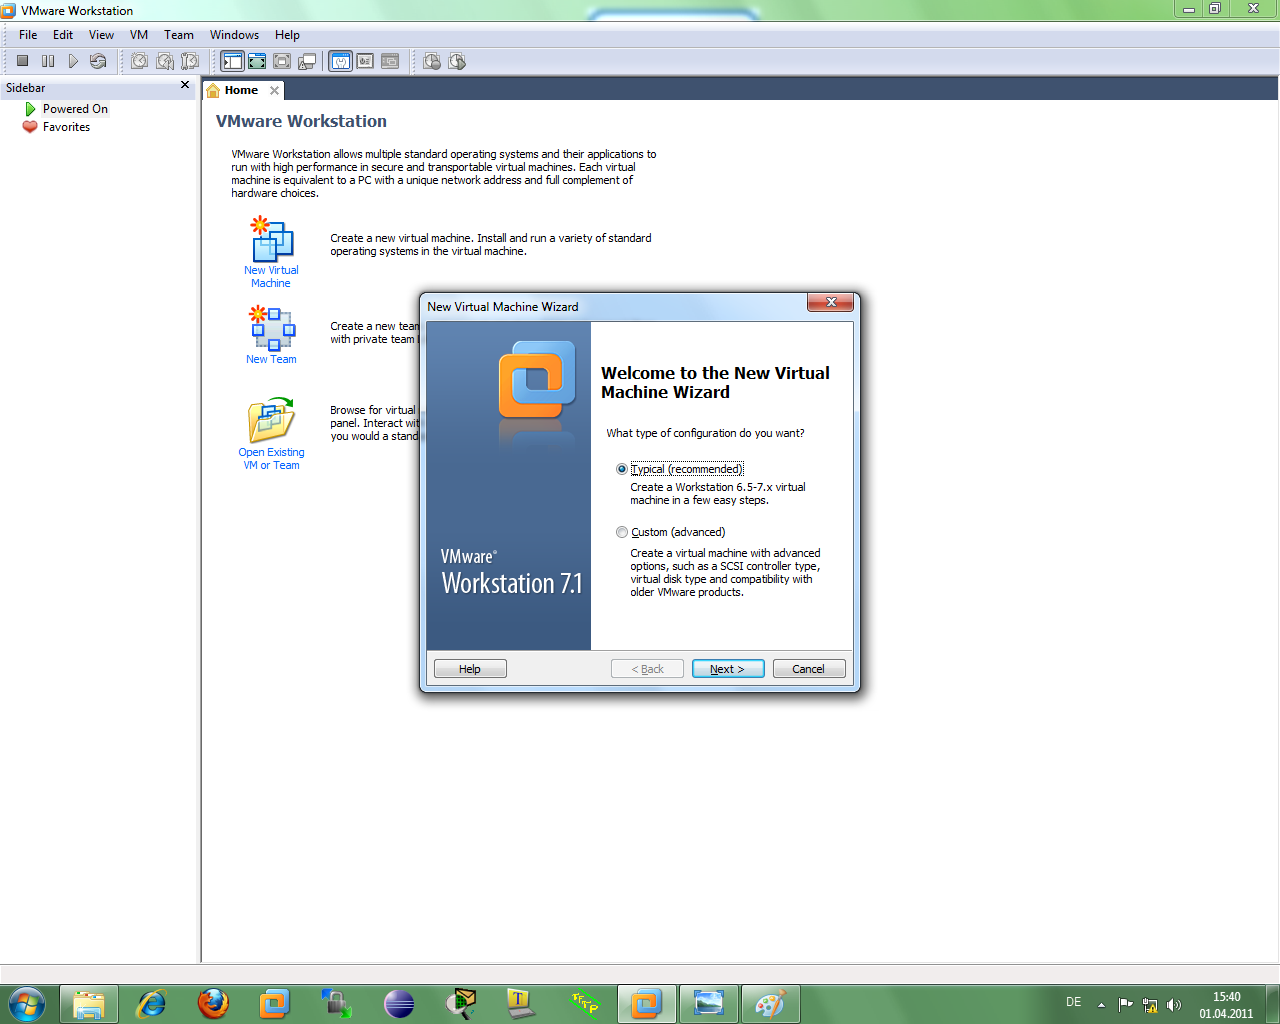
\includegraphics[width=0.75\textwidth]{screenshots/vm02.png}
\end{center}
\end{nofloat}

Hier muss die Option \textbf{I will install the operation system later} gewählt werden. Wieder geht es mit einem
Klick auf \textbf{Next} zur nächsten Seite.

\begin{nofloat}{figure}
\begin{center}
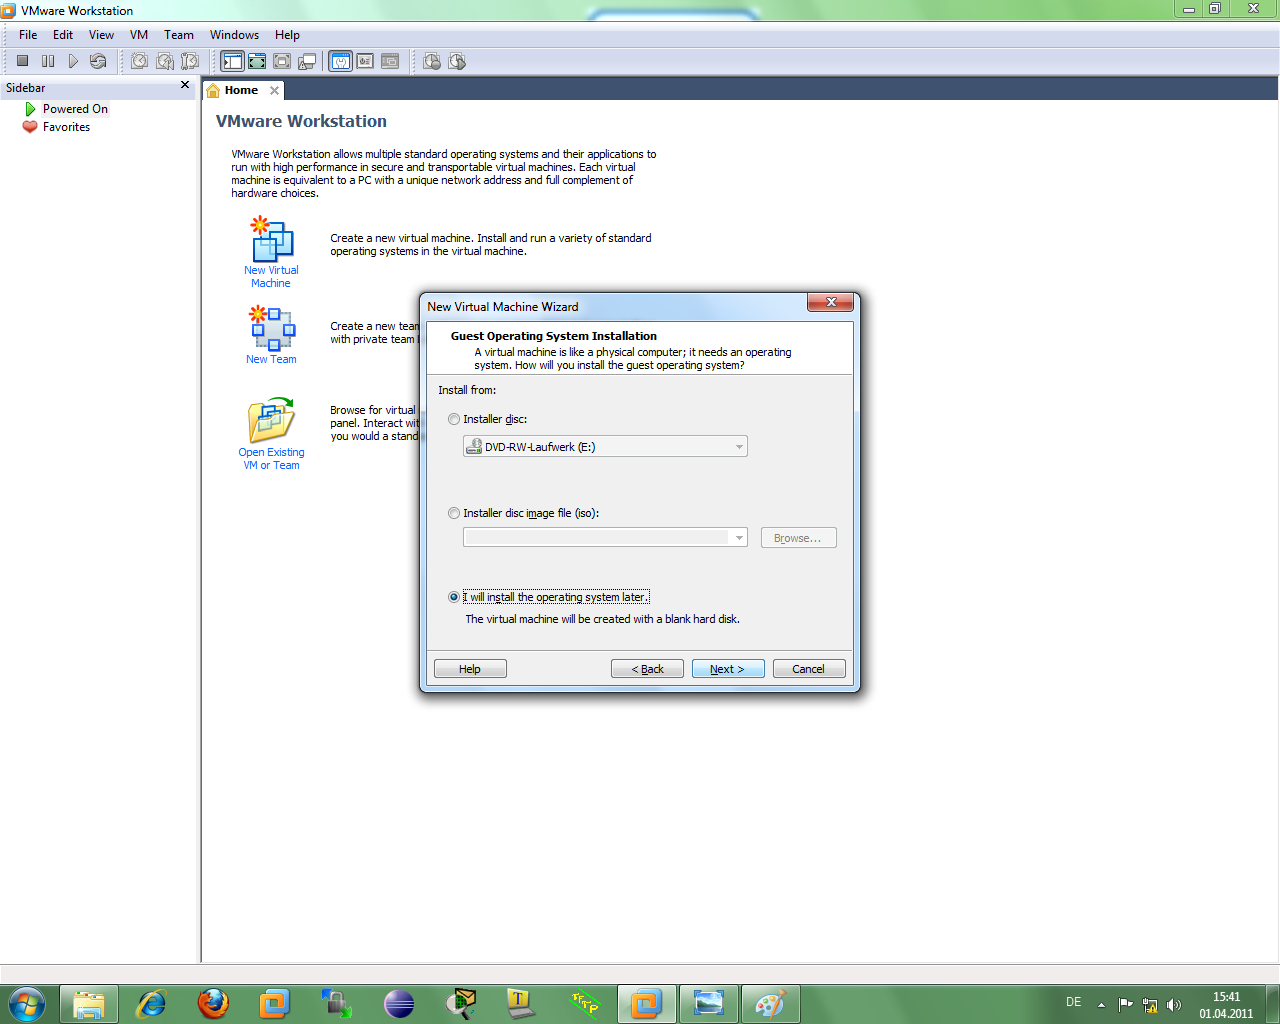
\includegraphics[width=0.75\textwidth]{screenshots/vm03.png}
\end{center}
\end{nofloat}

Wählen Sie nun als Betriebssystem \textbf{Linux} und als Version \textbf{Ubuntu} und bestätigen Sie diese
Eingaben mit einem Klick auf \textbf{Next}.

\begin{nofloat}{figure}
\begin{center}
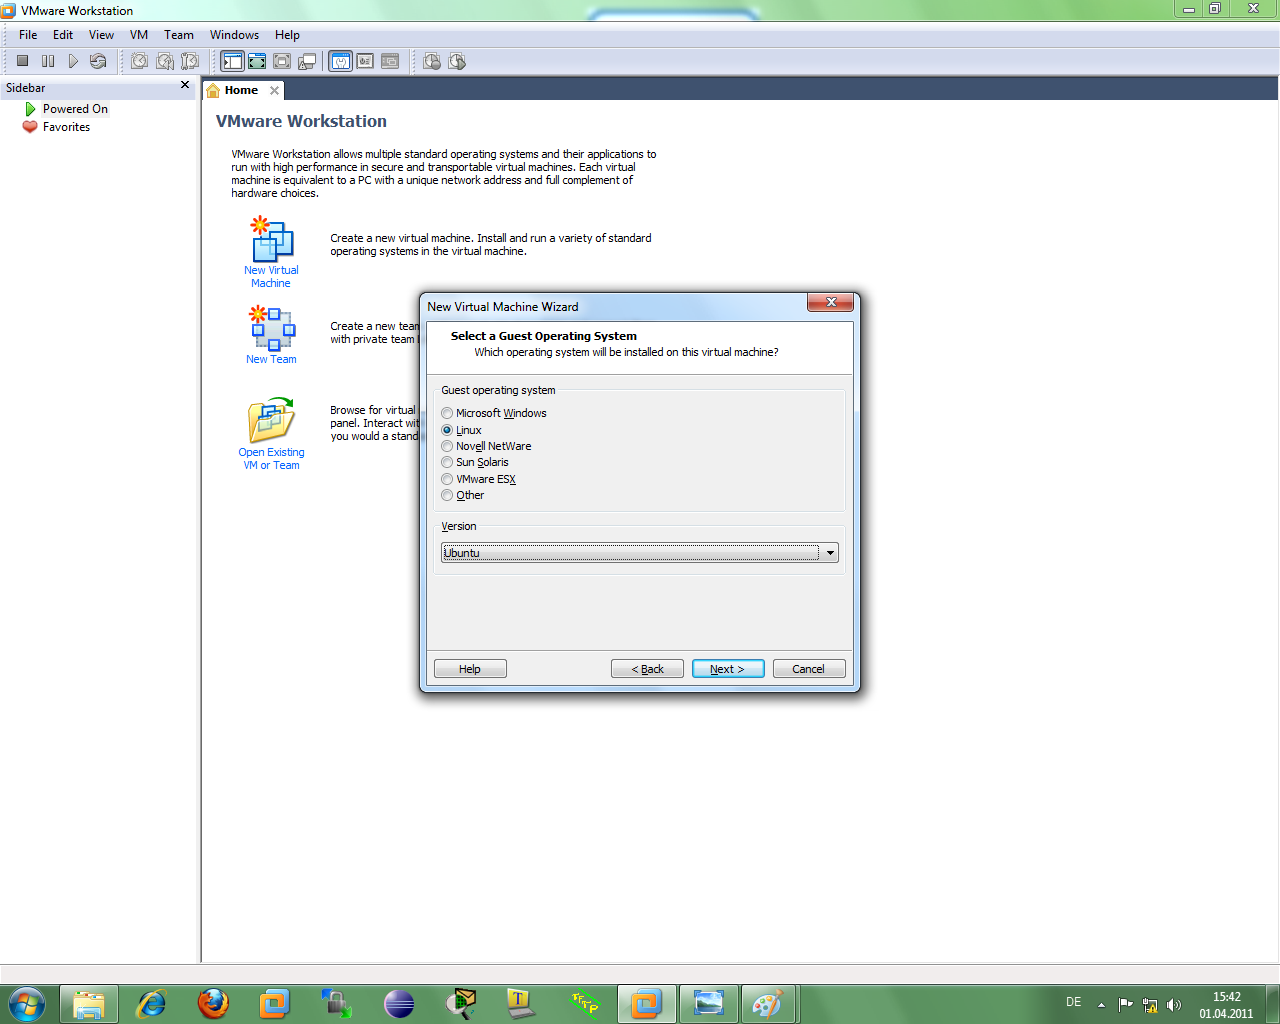
\includegraphics[width=0.75\textwidth]{screenshots/vm04.png}
\end{center}
\end{nofloat}

Geben Sie nun den Namen \textbf{srv200} und als Speicherort den Pfad \\
\textbf{D:$\backslash$Austausch$\backslash$Internetdienste$\backslash$srv200}
an.

\begin{nofloat}{figure}
\begin{center}
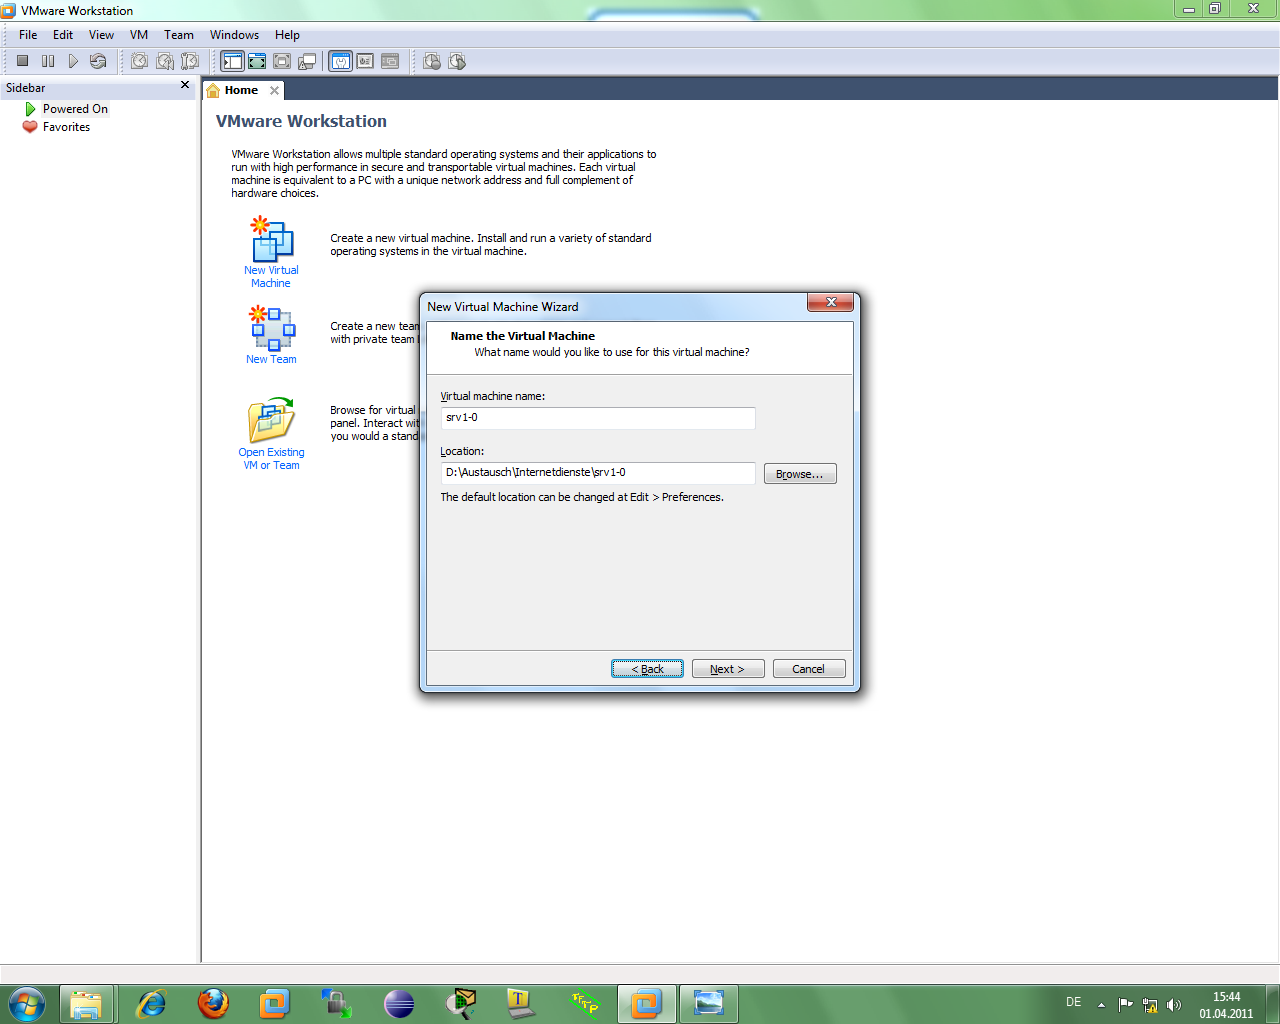
\includegraphics[width=0.75\textwidth]{screenshots/vm05.png}
\end{center}
\end{nofloat}

Für die Größe der virtuellen Festplatte wählen Sie bitte \textbf{8} Gigabyte.

\begin{nofloat}{figure}
\begin{center}
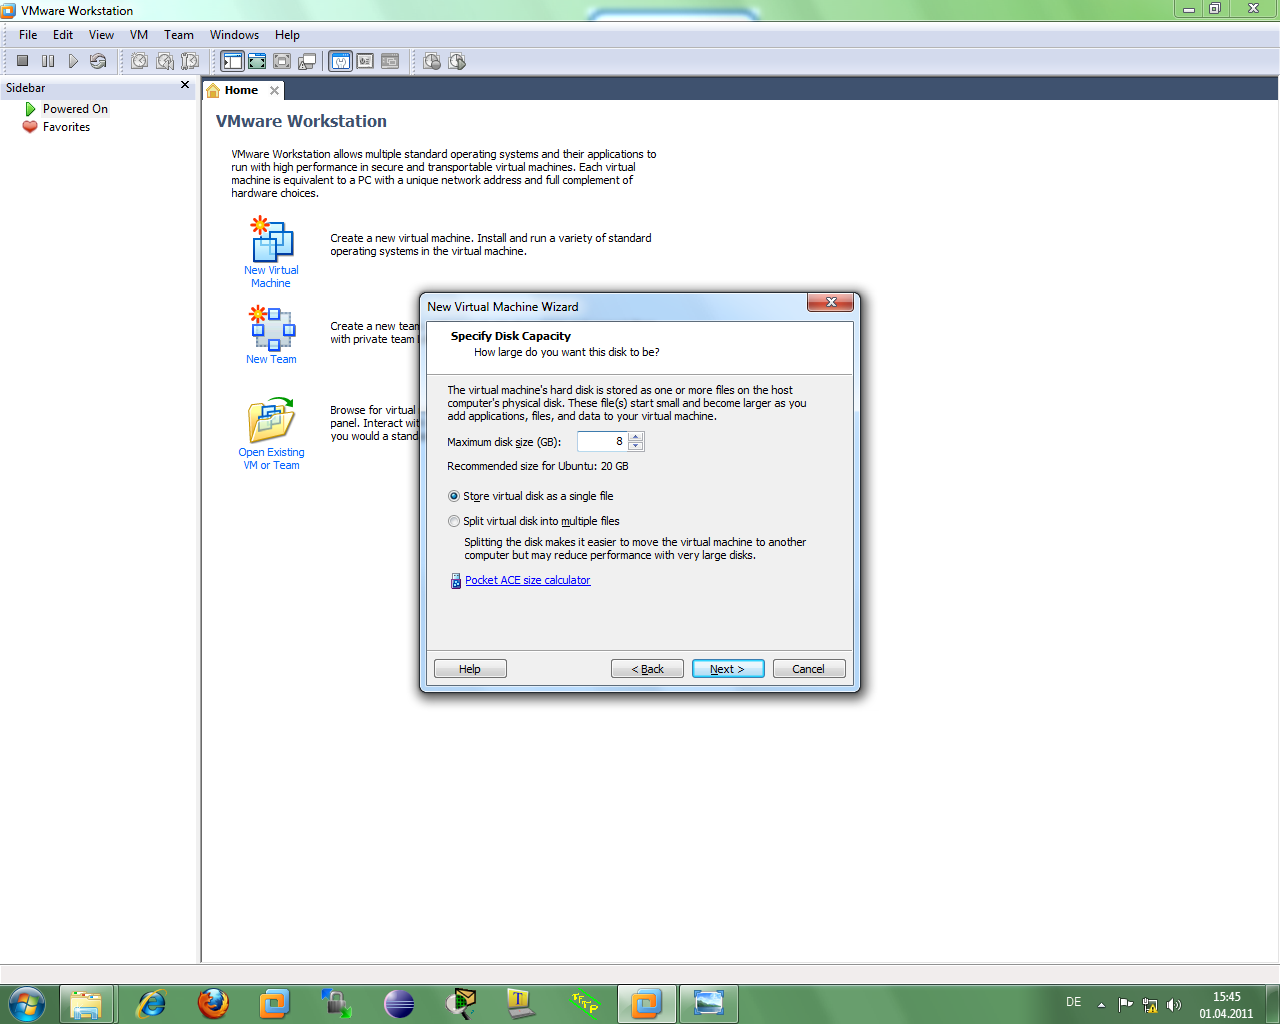
\includegraphics[width=0.75\textwidth]{screenshots/vm06.png}
\end{center}
\end{nofloat}

Der folgende Dialog wird jetzt mit \textbf{Finish} geschlossen.

\begin{nofloat}{figure}
\begin{center}
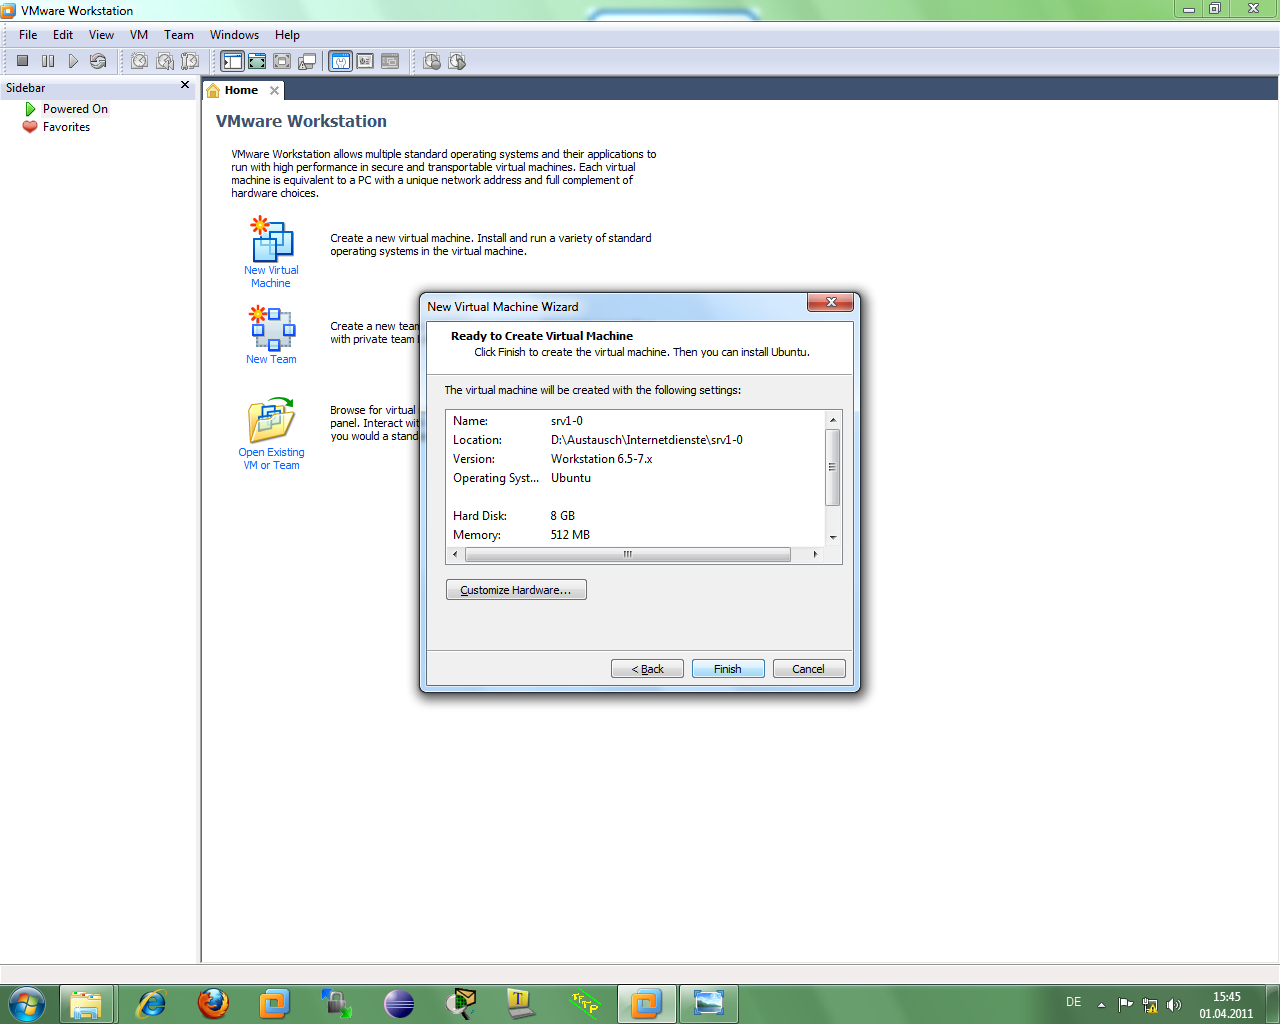
\includegraphics[width=0.75\textwidth]{screenshots/vm07.png}
\end{center}
\end{nofloat}

Als nächsten müssen noch einige Einstellungen der virtuellen Maschine bearbeitet werden. Hierzu wählen Sie
\textbf{Edit virtual machine settings}.

\begin{nofloat}{figure}
\begin{center}
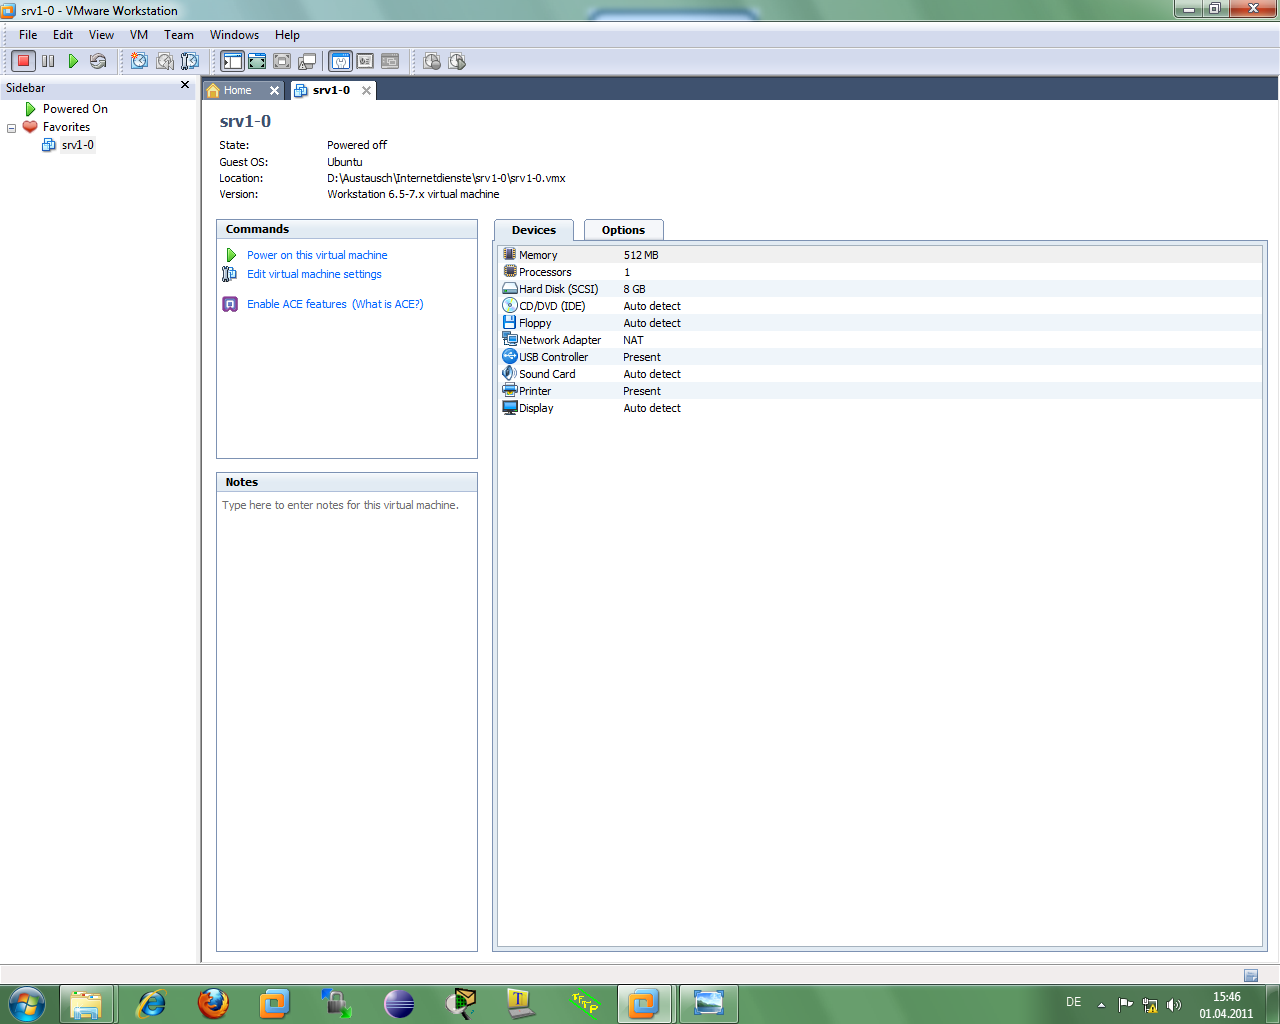
\includegraphics[width=0.75\textwidth]{screenshots/vm08.png}
\end{center}
\end{nofloat}

Wählen Sie nun den Eintrag \textbf{CD/DVD} und aktivieren Sie die Option \textbf{Use ISO image file}. Klicken Sie auf \textbf{Browse}
und wählen Sie die Datei \\ \textbf{D:$\backslash$Austausch$\backslash$Internetdienste$\backslash$ubuntu-10.10-server-i386.iso}.

\begin{nofloat}{figure}
\begin{center}
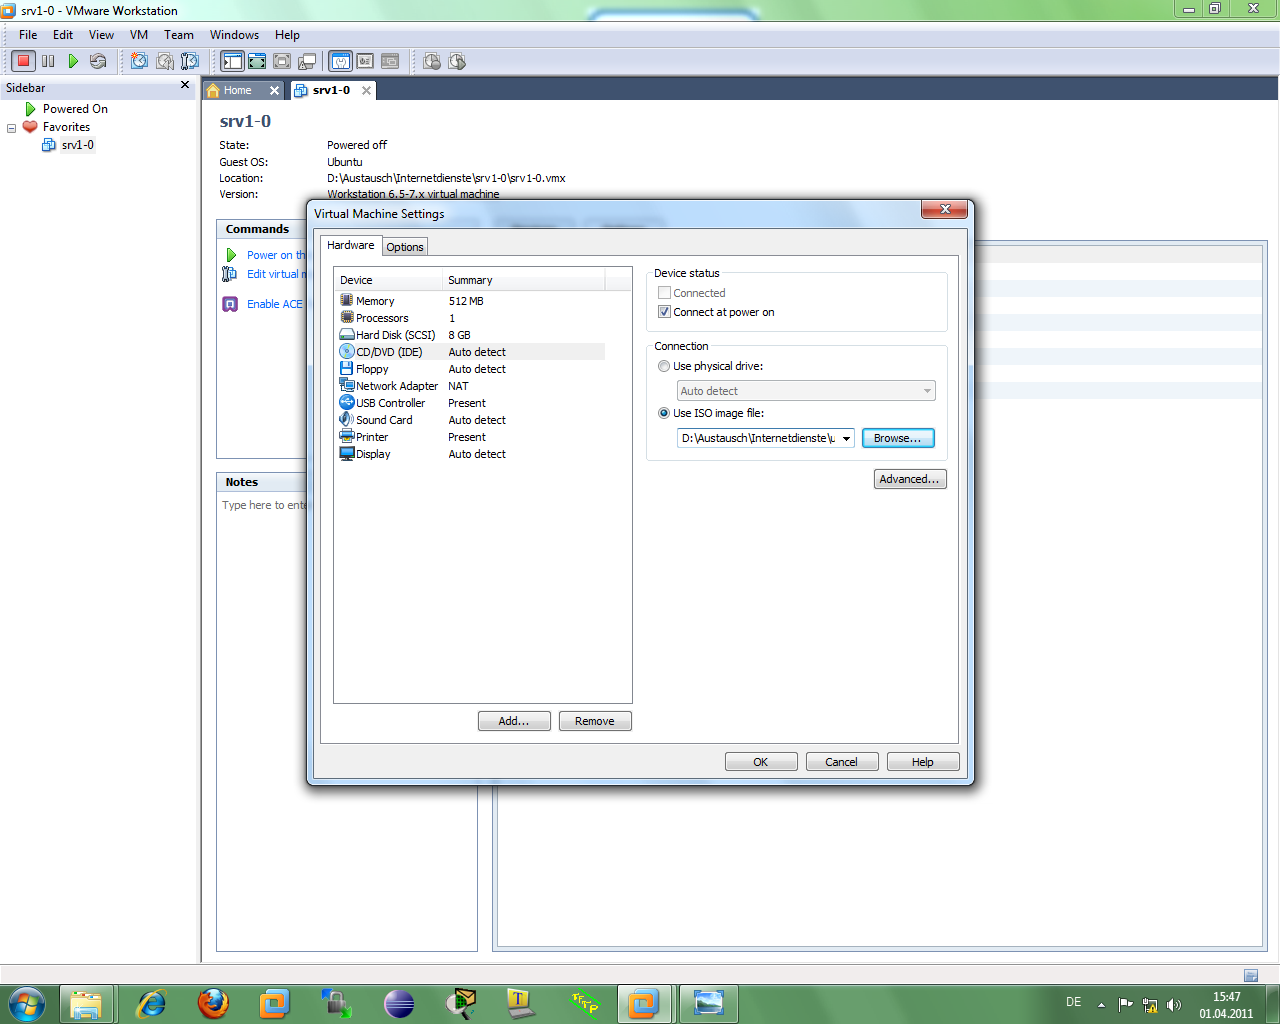
\includegraphics[width=0.75\textwidth]{screenshots/vm09.png}
\end{center}
\end{nofloat}

Danach wählen Sie den Eintrag \textbf{Network adapter} und aktivieren die Option
\textbf{Bridged}.

\begin{nofloat}{figure}
\begin{center}
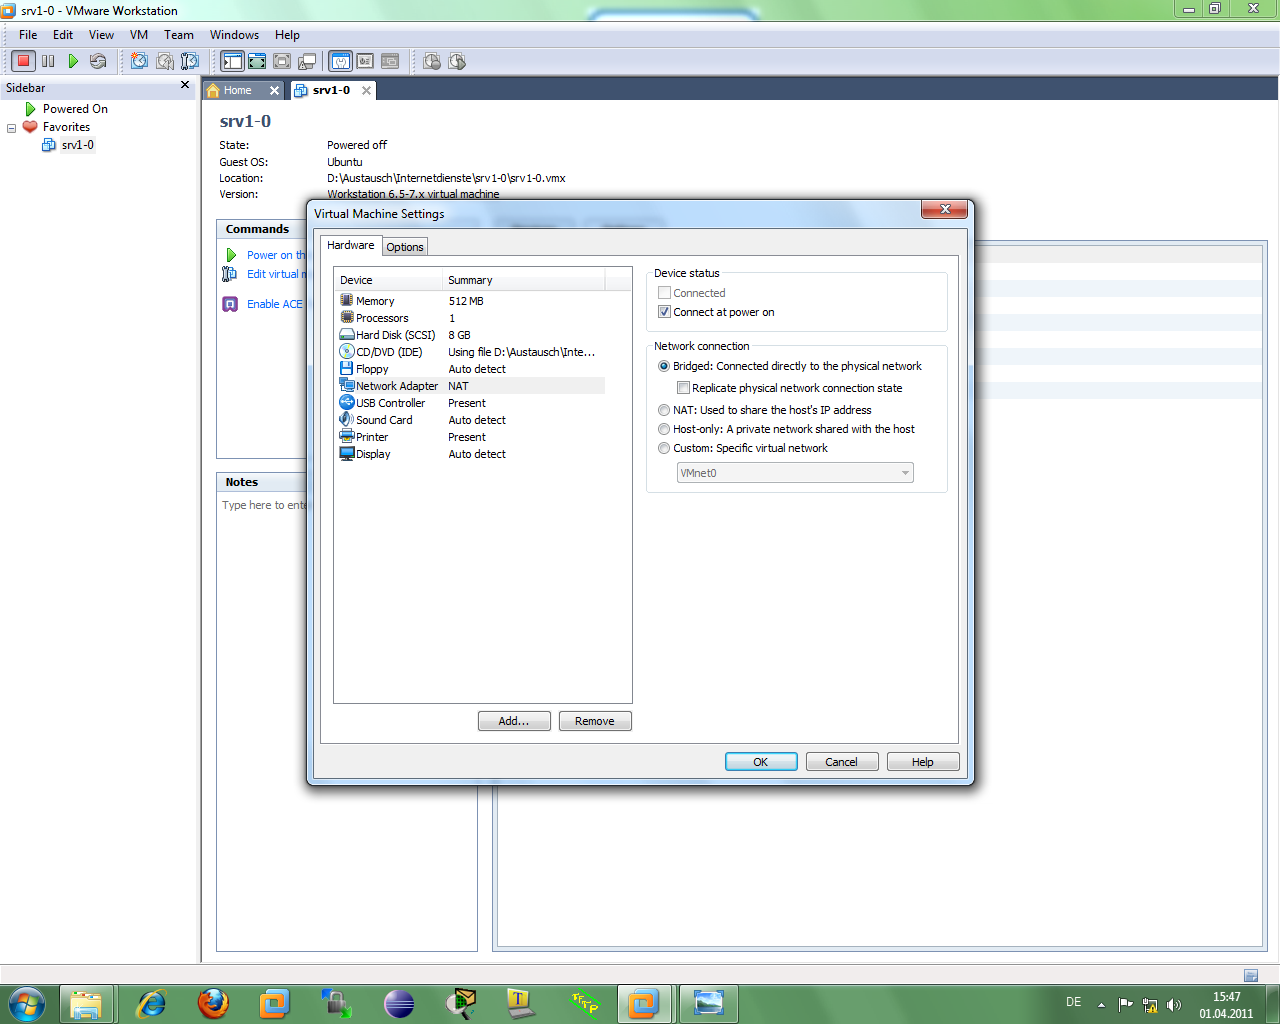
\includegraphics[width=0.75\textwidth]{screenshots/vm10.png}
\end{center}
\end{nofloat}

Verfahren Sie analog für den Server \textbf{srv201}.

%------------------------------------------------------------------------------
\subsection{Installation von Ubuntu}
%------------------------------------------------------------------------------
Nachdem Sie die virtuellen Maschinen gestartet haben, booten diese von dem zuvor angegebenen CD-Abbild. Wählen Sie zunächst die
englische Sprache aus. 
\begin{nofloat}{figure}
\begin{center}
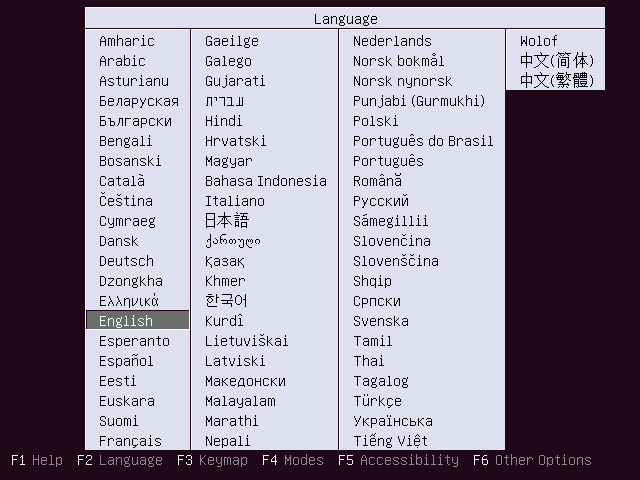
\includegraphics[width=0.75\textwidth]{screenshots/01_ubuntu_install.png}
\end{center}
\end{nofloat}

Danach den Eintrag \textbf{Install Ubuntu Server} wählen und mit der
Eingabe-Taste bestätigen.

\begin{nofloat}{figure}
\begin{center}
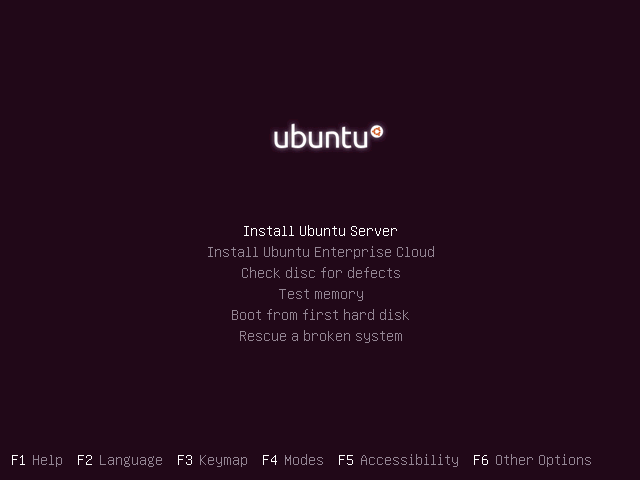
\includegraphics[width=0.75\textwidth]{screenshots/02_ubuntu_install.png}
\end{center}
\end{nofloat}

Um den Installationsprozess in englischer Sprache zu durchlaufen, hier die
Sprache \textbf{English} wählen.

\begin{nofloat}{figure}
\begin{center}
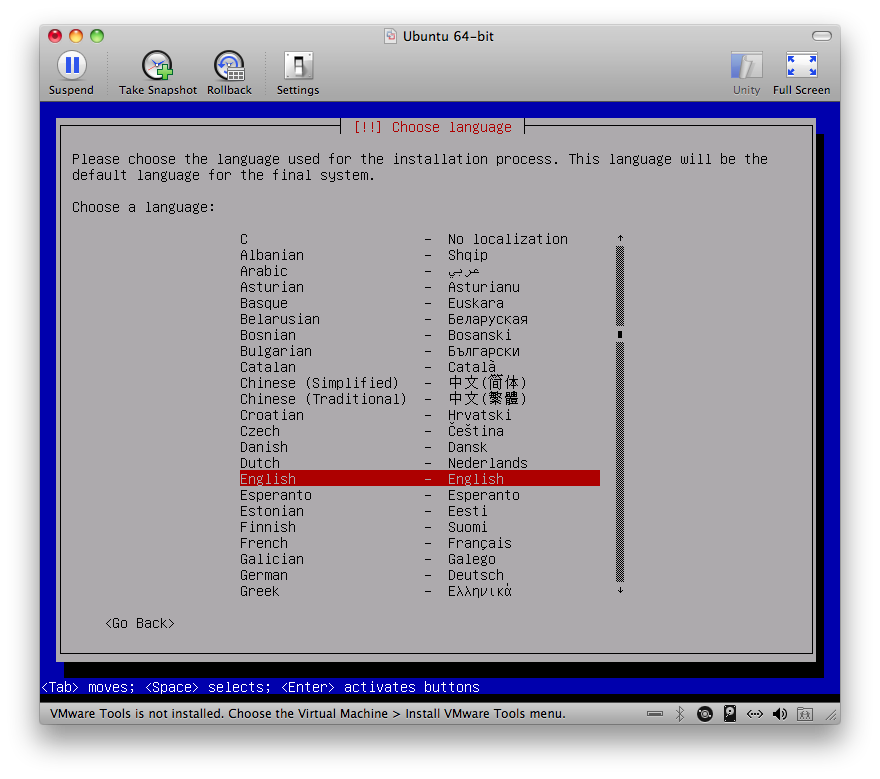
\includegraphics[width=0.75\textwidth]{screenshots/03_ubuntu_install.png}
\end{center}
\end{nofloat}

Die Zeitzone und Region für die Tasturbelegung wird \textbf{Europe} ausgewählt.

\begin{nofloat}{figure}
\begin{center}
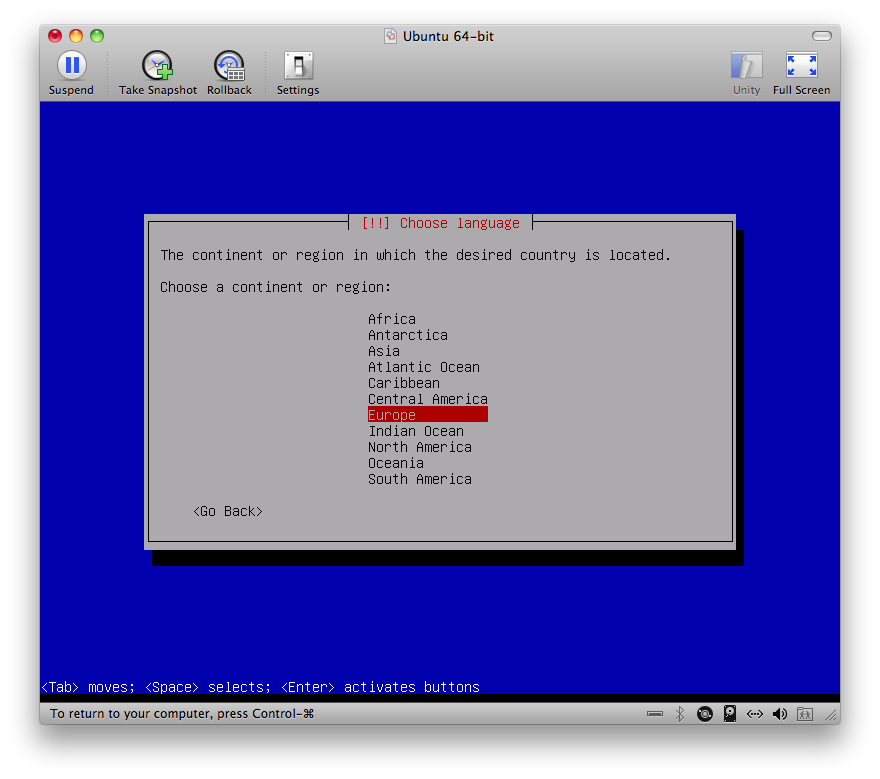
\includegraphics[width=0.75\textwidth]{screenshots/04_ubuntu_install.png}
\end{center}
\end{nofloat}
\newpage
Im nächsten Dialog als Land \textbf{Germany} auswählen.

\begin{nofloat}{figure}
\begin{center}
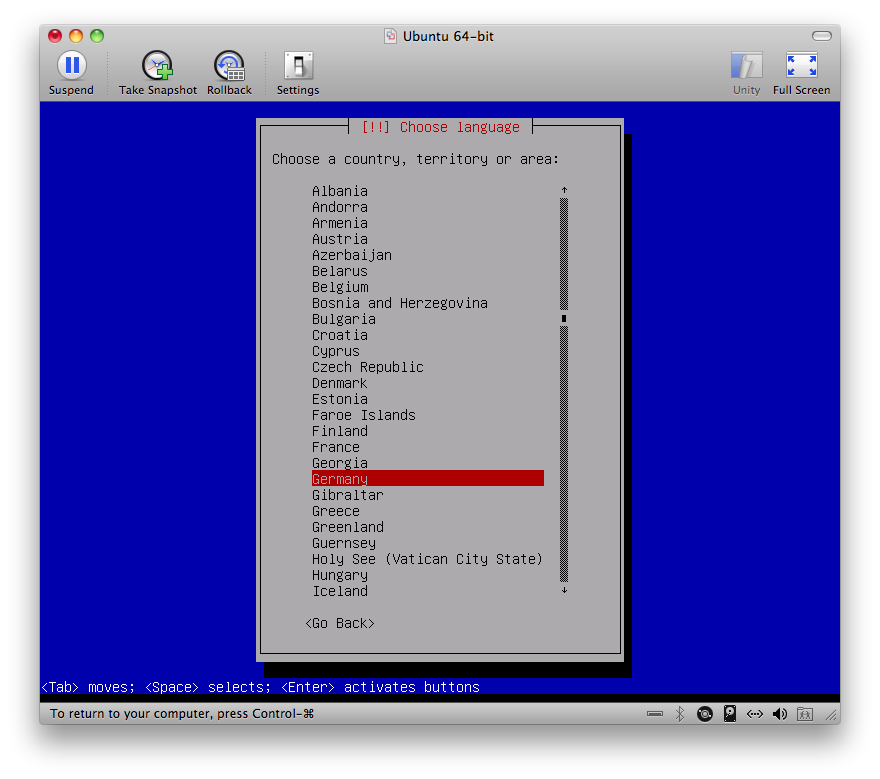
\includegraphics[width=0.75\textwidth]{screenshots/05_ubuntu_install.png}
\end{center}
\end{nofloat}

Als nächster Schritt wird die Tastatur-Belegung angegeben. Sie können diese automatisch erkennen lassen. Hierzu müssen Sie in
den folgenden Dialogen verschiedene Tasten drücken.

\begin{nofloat}{figure}
\begin{center}
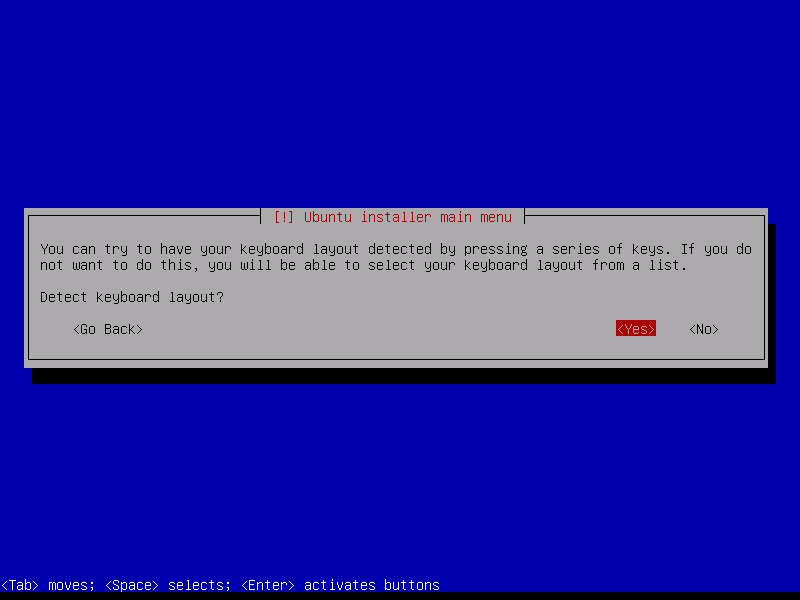
\includegraphics[width=0.75\textwidth]{screenshots/06_ubuntu_install.png}
\end{center}
\end{nofloat}

\begin{nofloat}{figure}
\begin{center}
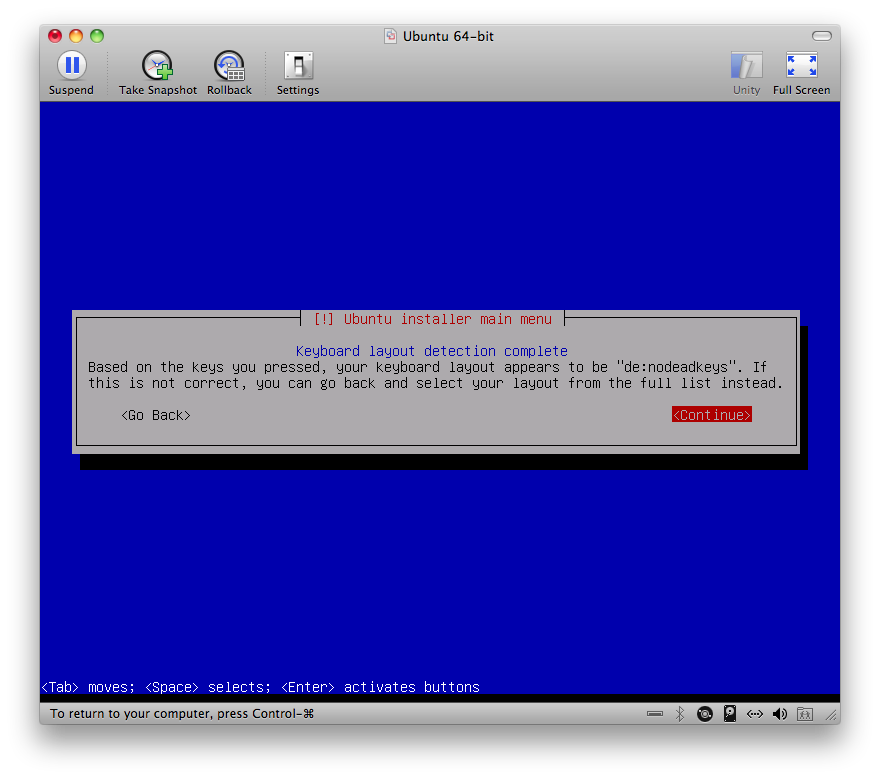
\includegraphics[width=0.75\textwidth]{screenshots/07_ubuntu_install.png}
\end{center}
\end{nofloat}

\begin{nofloat}{figure}
\begin{center}
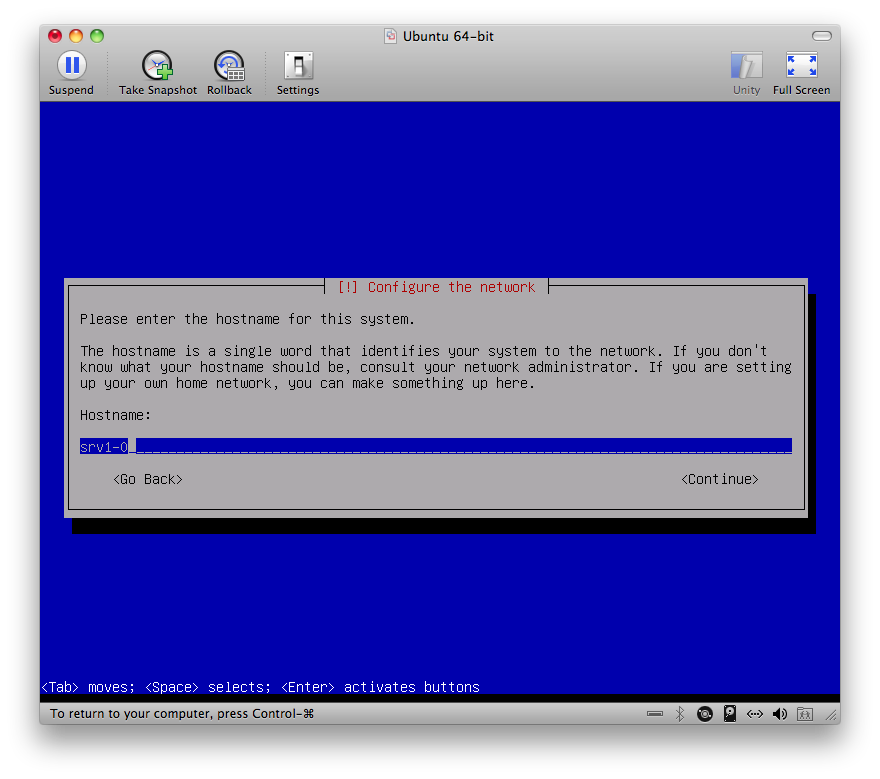
\includegraphics[width=0.75\textwidth]{screenshots/08_ubuntu_install.png}
\end{center}
\end{nofloat}

\begin{nofloat}{figure}
\begin{center}
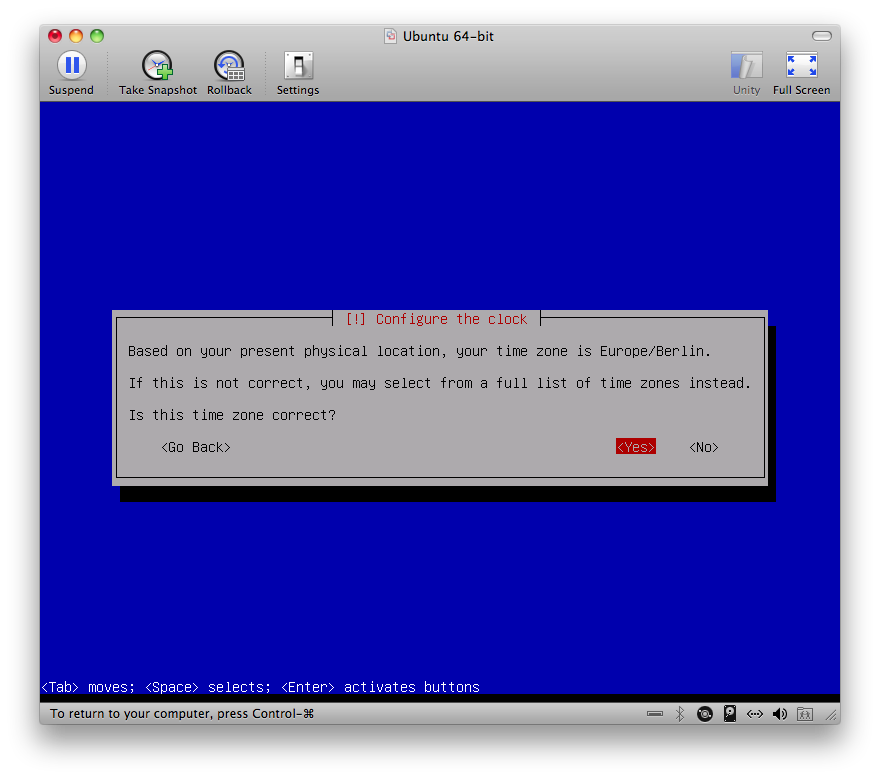
\includegraphics[width=0.75\textwidth]{screenshots/09_ubuntu_install.png}
\end{center}
\end{nofloat}

Nach der Hardware- und Netzwerk-Erkennung können Sie nun einen Hostnamen
eintragen. Geben Sie hier bitte \textbf{srv200} an.

\begin{nofloat}{figure}
\begin{center}
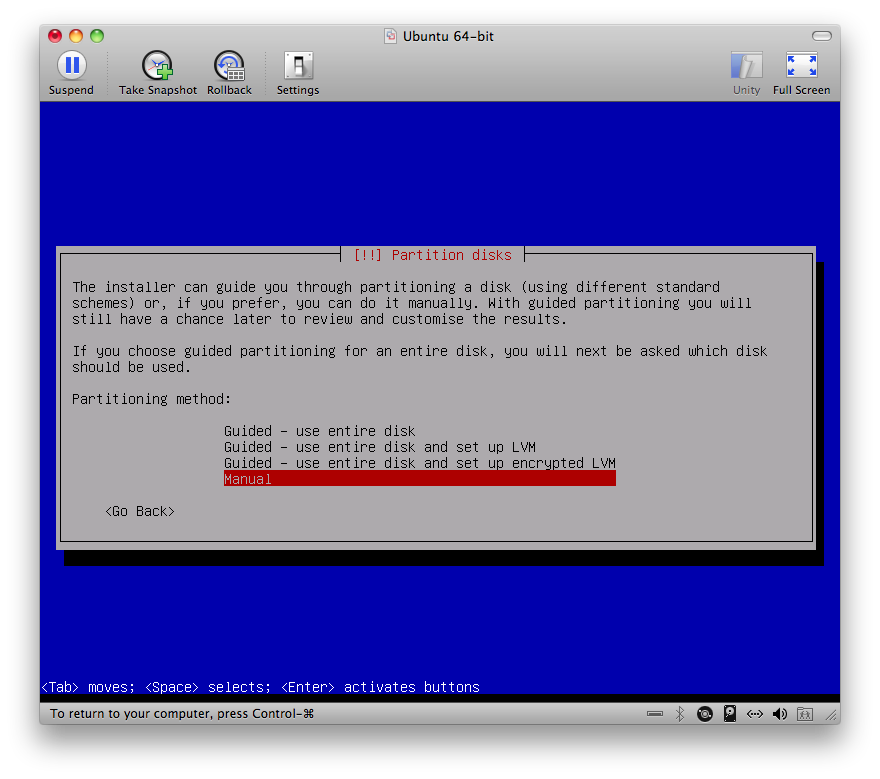
\includegraphics[width=0.75\textwidth]{screenshots/10_ubuntu_install.png}
\end{center}
\end{nofloat}
\newpage
Nun wird die Festplatte partitioniert. Wählen Sie hier den Eintrag
\textbf{Manual}.

\begin{nofloat}{figure}
\begin{center}
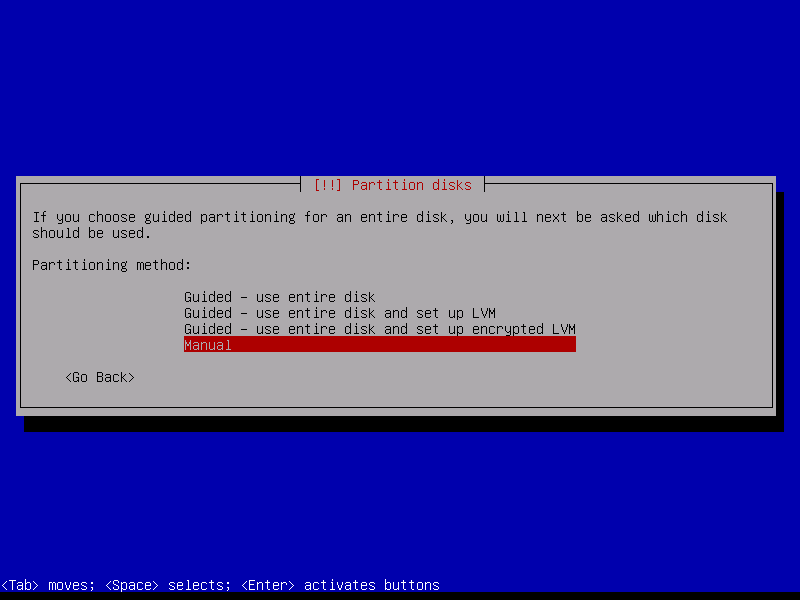
\includegraphics[width=0.75\textwidth]{screenshots/11_ubuntu_install.png}
\end{center}
\end{nofloat}

Hier nun den Eintrag \textbf{SCSI3} wählen.

\begin{nofloat}{figure}
\begin{center}
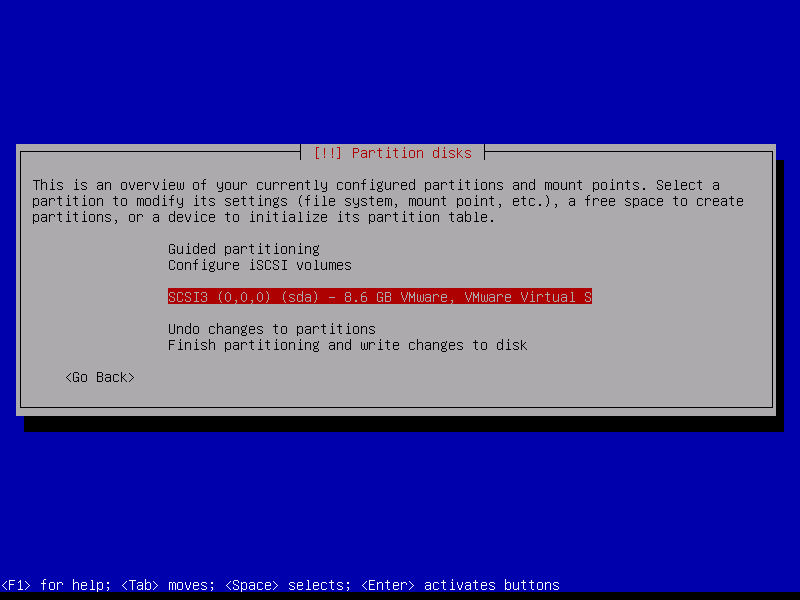
\includegraphics[width=0.75\textwidth]{screenshots/12_ubuntu_install.png}
\end{center}
\end{nofloat}
\newpage
Erzeugen Sie eine neue leere Partitionstabelle.

\begin{nofloat}{figure}
\begin{center}
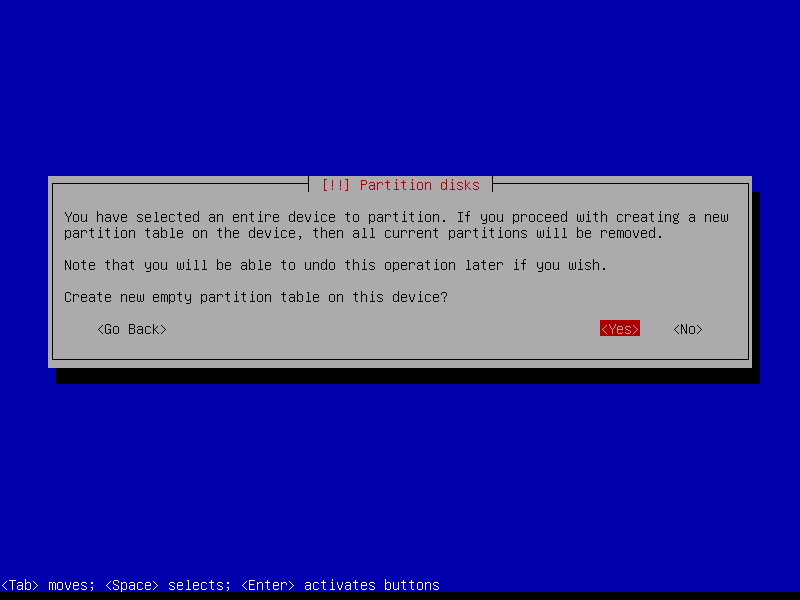
\includegraphics[width=0.75\textwidth]{screenshots/13_ubuntu_install.png}
\end{center}
\end{nofloat}

Wählen Sie hier nun \textbf{FREE SPACE} aus.

\begin{nofloat}{figure}
\begin{center}
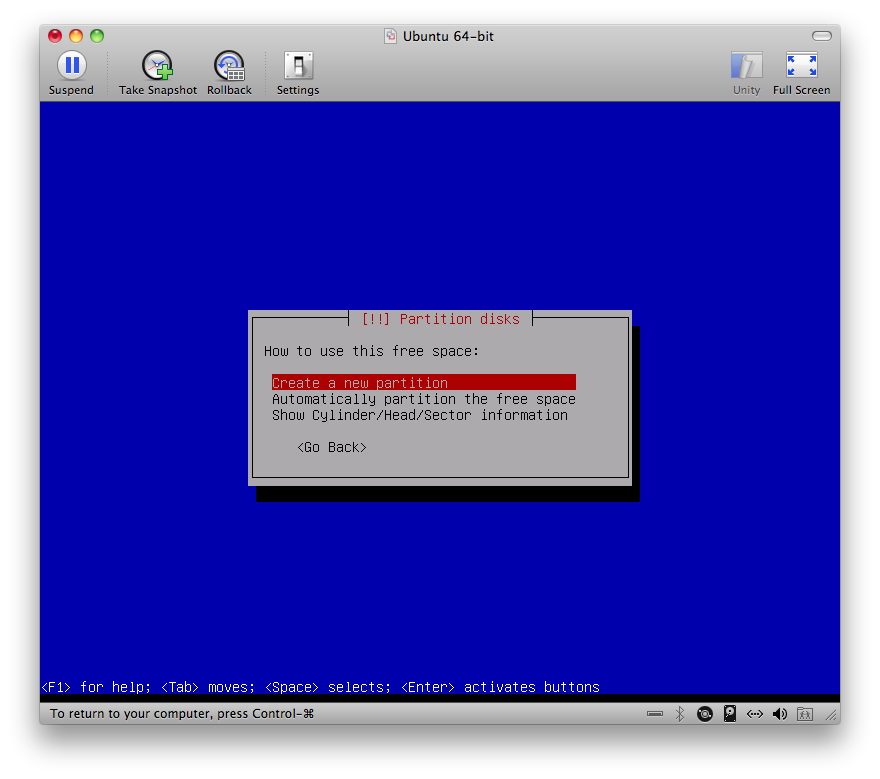
\includegraphics[width=0.75\textwidth]{screenshots/14_ubuntu_install.png}
\end{center}
\end{nofloat}
\newpage
Hier nun \textbf{Create a new partition} wählen.

\begin{nofloat}{figure}
\begin{center}
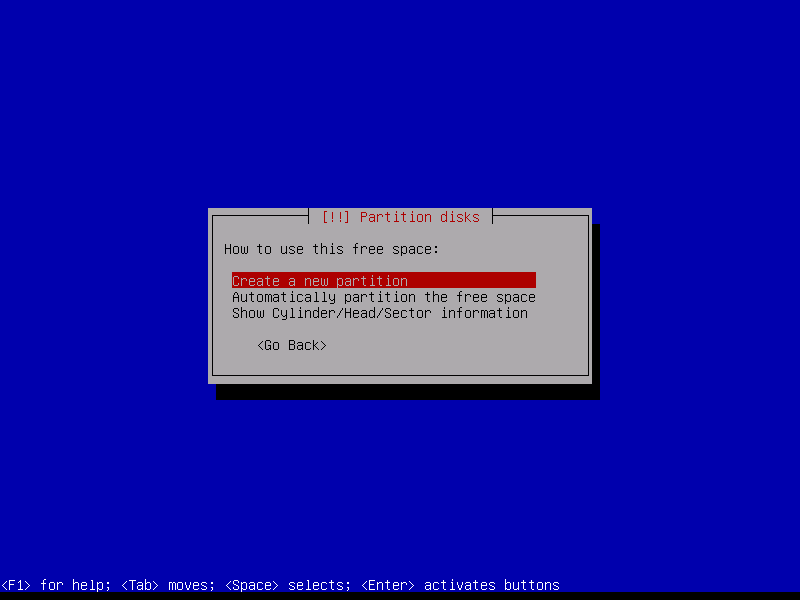
\includegraphics[width=0.75\textwidth]{screenshots/15_ubuntu_install.png}
\end{center}
\end{nofloat}

Die erste Partition wird zum Auslagern verwendet und wird mit 0,5 GB angegeben.

\begin{nofloat}{figure}
\begin{center}
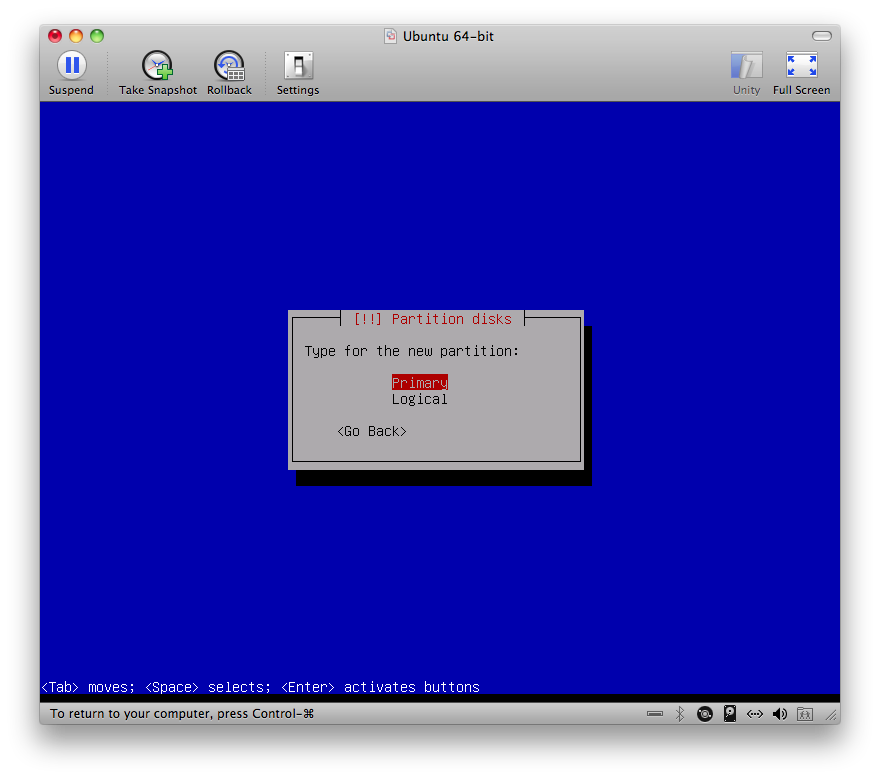
\includegraphics[width=0.75\textwidth]{screenshots/16_ubuntu_install.png}
\end{center}
\end{nofloat}
\newpage
Die Partition wird als primäre Partition angelegt. Wählen Sie hier
\textbf{Primary} aus.

\begin{nofloat}{figure}
\begin{center}
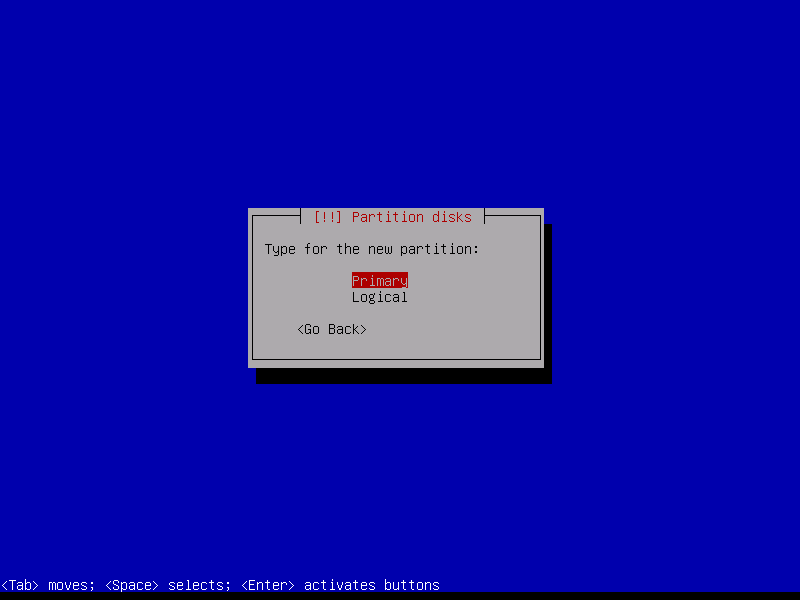
\includegraphics[width=0.75\textwidth]{screenshots/17_ubuntu_install.png}
\end{center}
\end{nofloat}

Im nächsten Schritt \textbf{Beginning} auswählen um die Partition am Anfang zu
erstellen.

\begin{nofloat}{figure}
\begin{center}
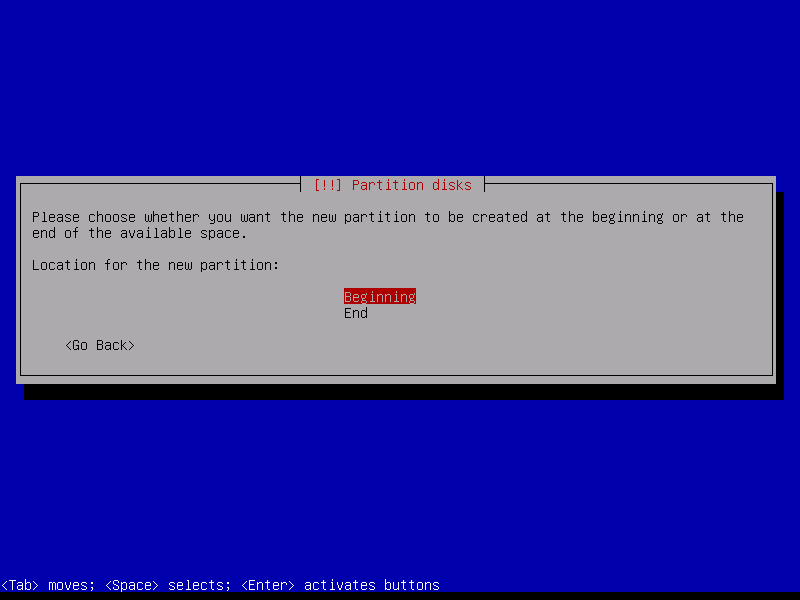
\includegraphics[width=0.75\textwidth]{screenshots/18_ubuntu_install.png}
\end{center}
\end{nofloat}
\newpage
Oben als Partitionseinstellung den Typ \textbf{swap area} auswählen. Danach
\textbf{Done setting up the partition} wählen.

\begin{nofloat}{figure}
\begin{center}
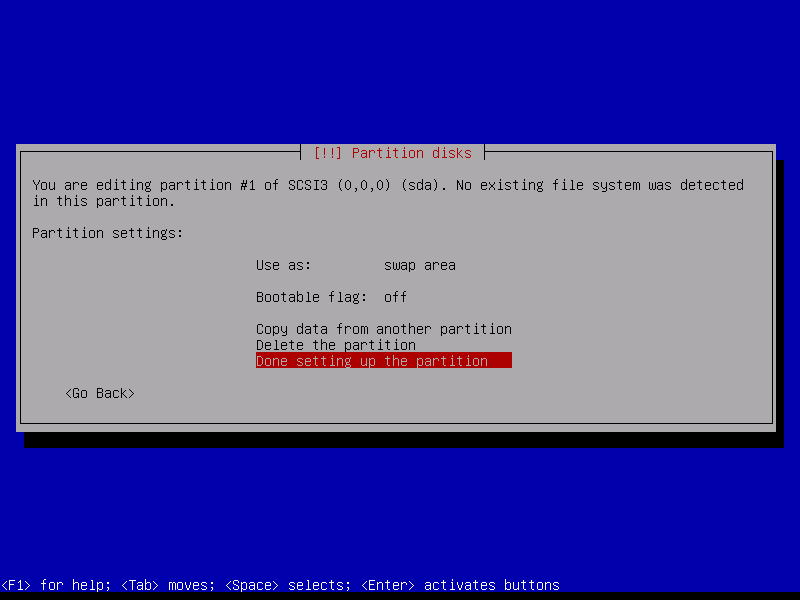
\includegraphics[width=0.75\textwidth]{screenshots/19_ubuntu_install.png}
\end{center}
\end{nofloat}

Als nächstes eine Partition für das System anlegen. Dazu wiederholt
\textbf{FREE SPACE} auswählen.

\begin{nofloat}{figure}
\begin{center}
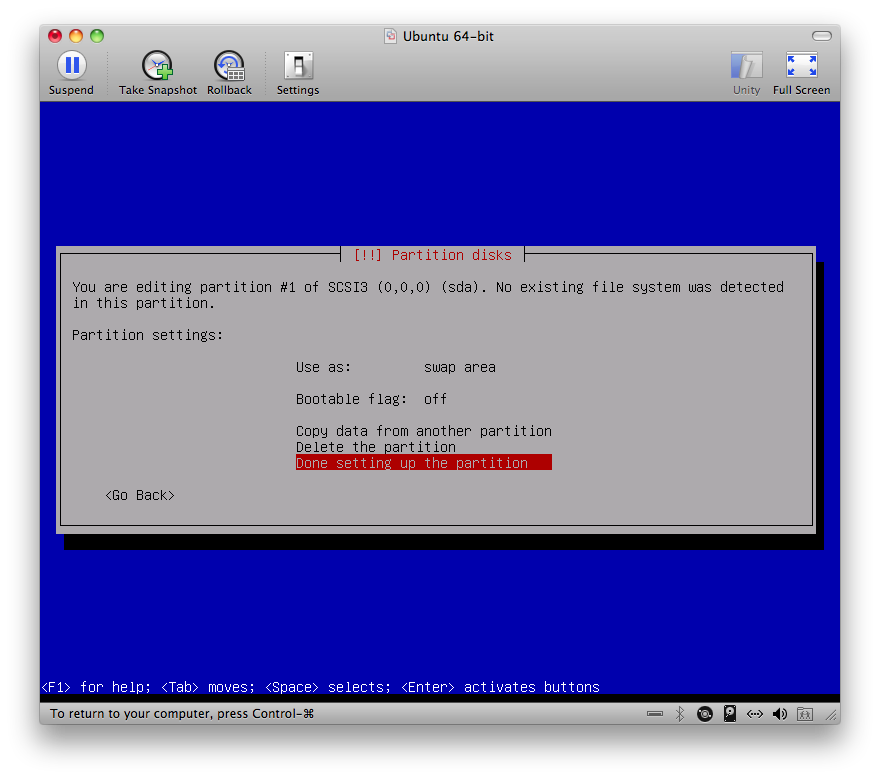
\includegraphics[width=0.75\textwidth]{screenshots/20_ubuntu_install.png}
\end{center}
\end{nofloat}
\newpage
Wiederholt \textbf{Create a new partition} auswählen.

\begin{nofloat}{figure}
\begin{center}
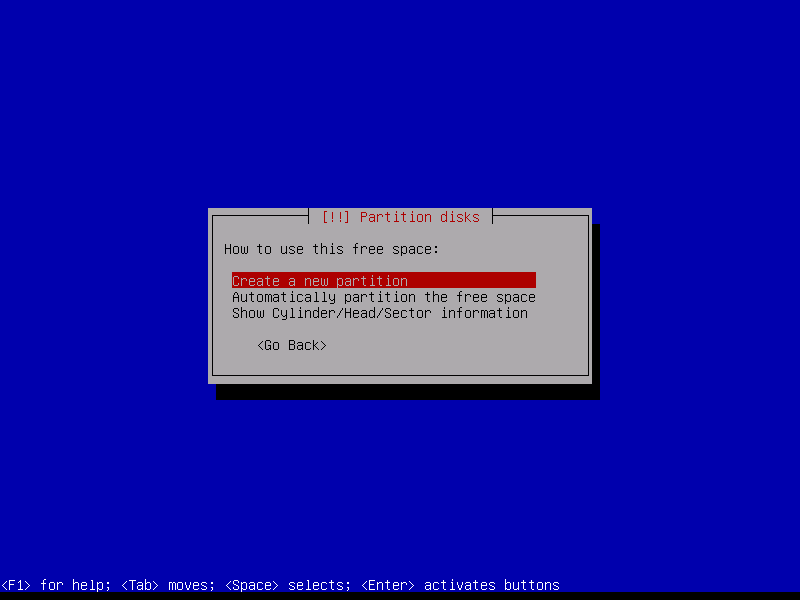
\includegraphics[width=0.75\textwidth]{screenshots/21_ubuntu_install.png}
\end{center}
\end{nofloat}

Hier den restlichen Speicher auswählen und den vorgeschlagenen Wert übernehmen.

\begin{nofloat}{figure}
\begin{center}
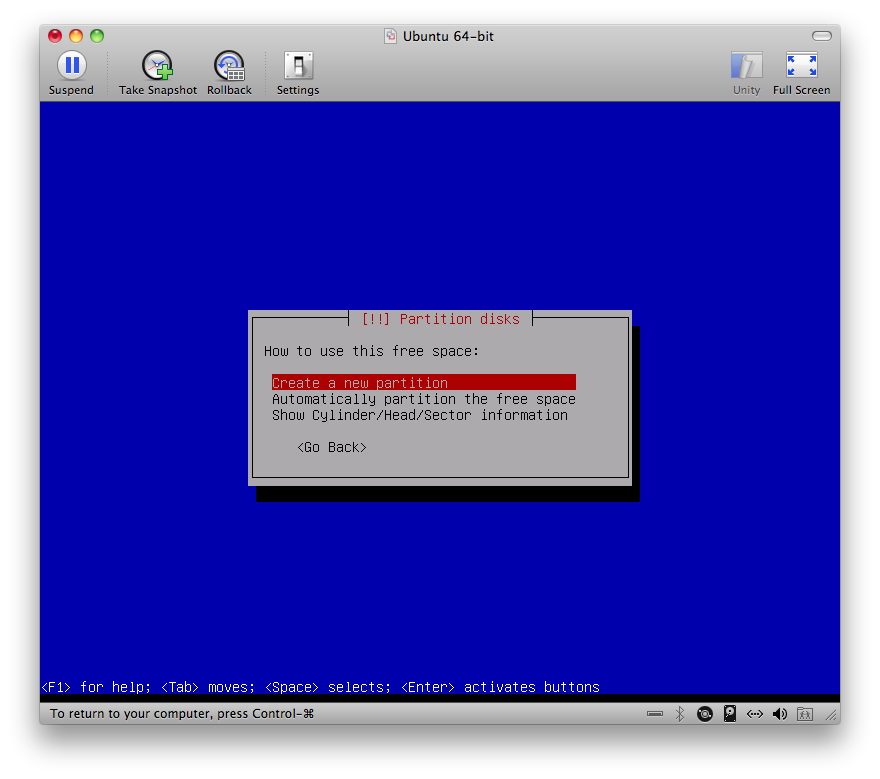
\includegraphics[width=0.75\textwidth]{screenshots/22_ubuntu_install.png}
\end{center}
\end{nofloat}
\newpage

Wiederholt die Partition vom Typ \textbf{Primary} anlegen.


\begin{nofloat}{figure}
\begin{center}
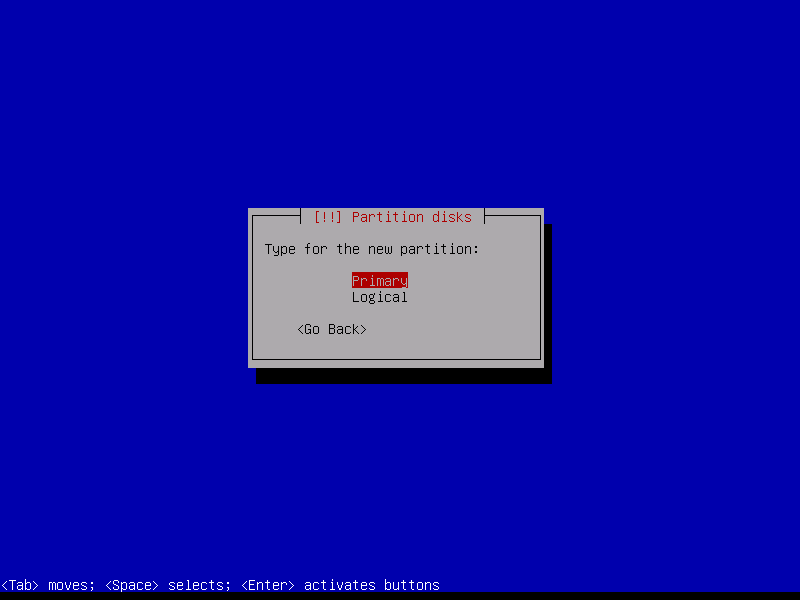
\includegraphics[width=0.75\textwidth]{screenshots/23_ubuntu_install.png}
\end{center}
\end{nofloat}

Als Partitionstyp wird der Vorschlag \textbf{Ext4} angegeben und mit
\textbf{Done setting up the partition} beenden.

\begin{nofloat}{figure}
\begin{center}
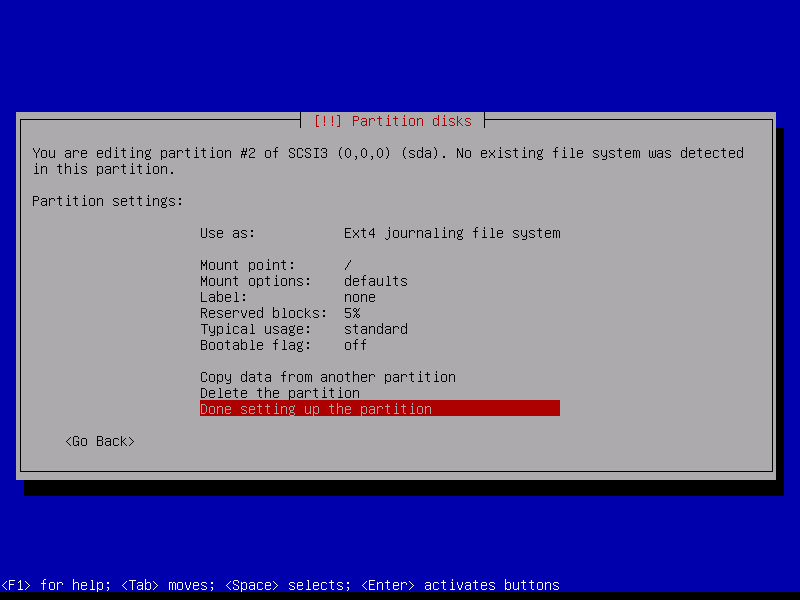
\includegraphics[width=0.75\textwidth]{screenshots/24_ubuntu_install.png}
\end{center}
\end{nofloat}
\newpage
Die Partitionierung ist abgeschlossen und wird mit \textbf{Finish partitioning
and write changes to disk} beendet.

\begin{nofloat}{figure}
\begin{center}
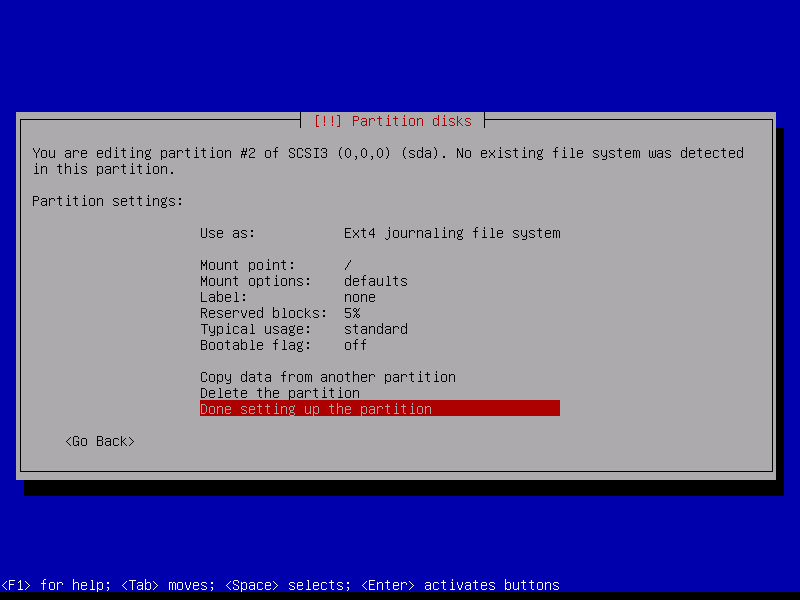
\includegraphics[width=0.75\textwidth]{screenshots/25_ubuntu_install.png}
\end{center}
\end{nofloat}

\begin{nofloat}{figure}
\begin{center}
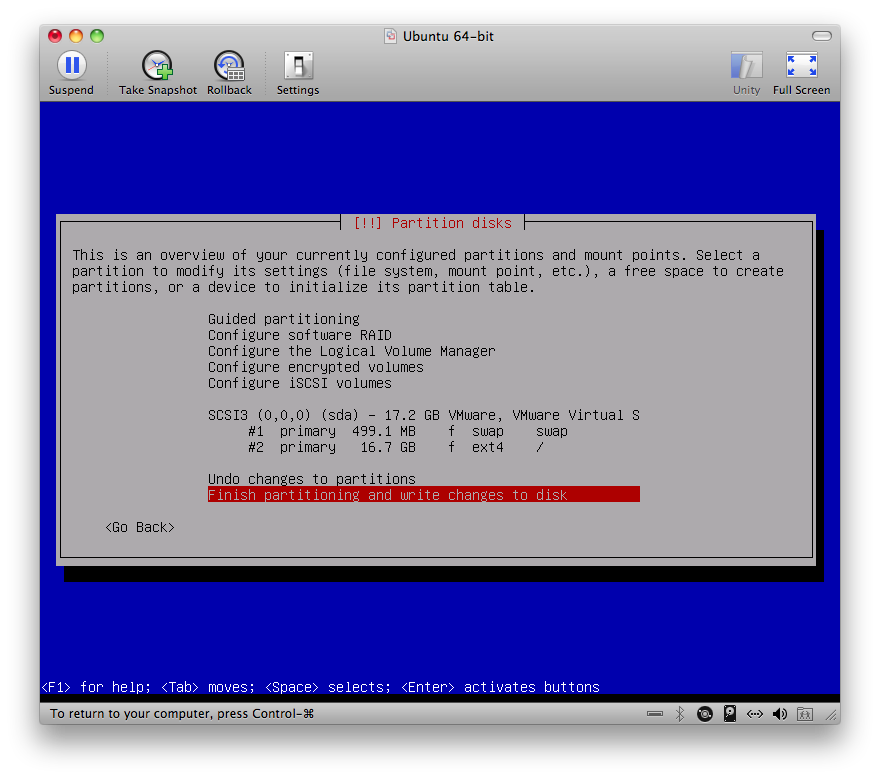
\includegraphics[width=0.75\textwidth]{screenshots/26_ubuntu_install.png}
\end{center}
\end{nofloat}
\newpage
Jetzt kann ein Benutzer angelegt werden. Für \textbf{srv200} wählen wir den
Namen \textbf{admin1}.

\begin{nofloat}{figure}
\begin{center}
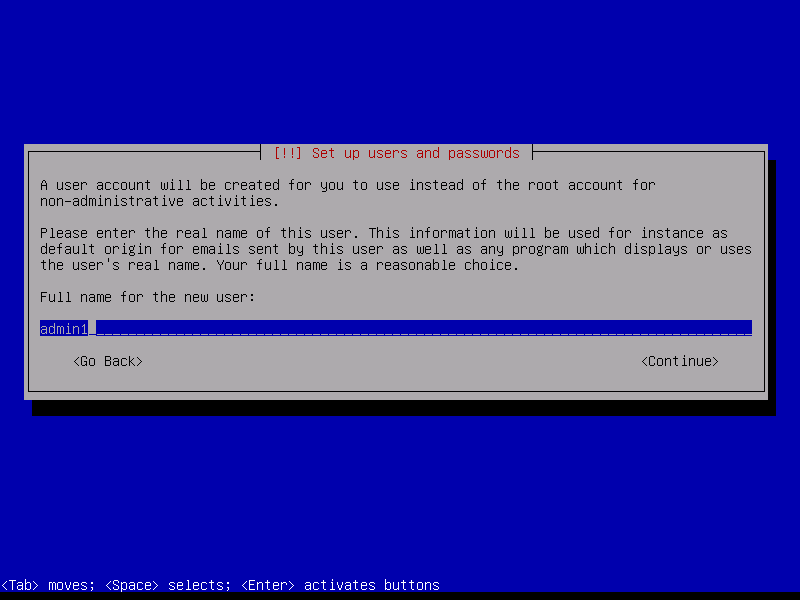
\includegraphics[width=0.75\textwidth]{screenshots/27_ubuntu_install.png}
\end{center}
\end{nofloat}

\begin{nofloat}{figure}
\begin{center}
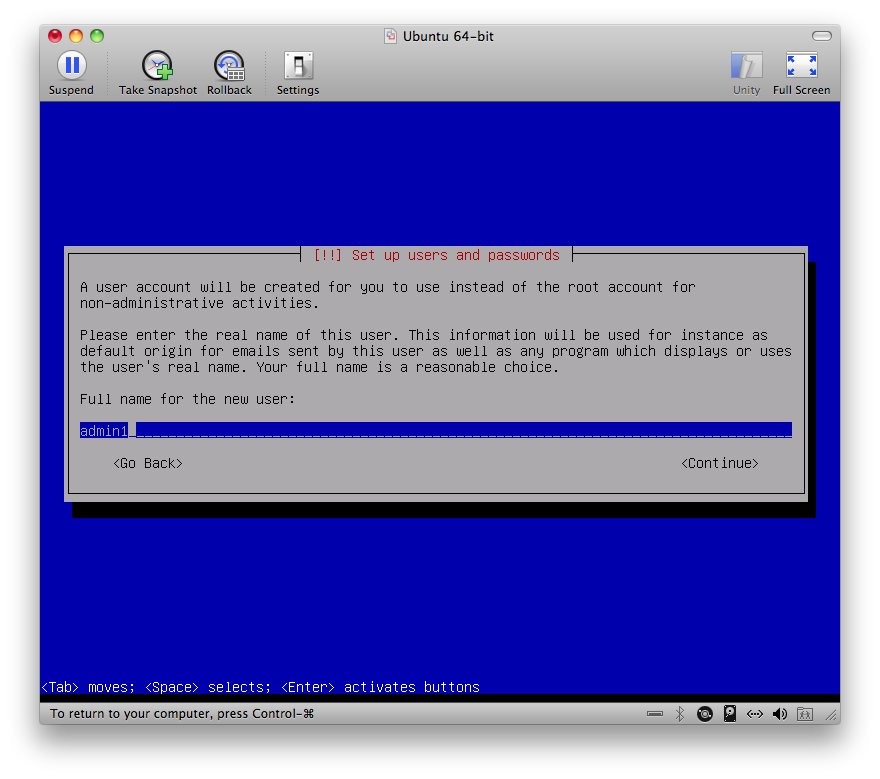
\includegraphics[width=0.75\textwidth]{screenshots/28_ubuntu_install.png}
\end{center}
\end{nofloat}
\newpage
Als Passwort vergeben wir hier \textbf{password1}.

\begin{nofloat}{figure}
\begin{center}
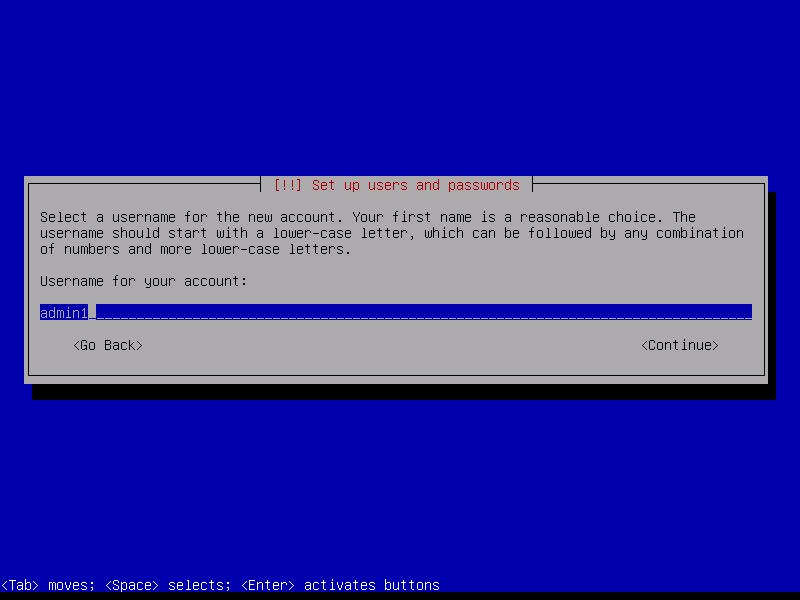
\includegraphics[width=0.75\textwidth]{screenshots/29_ubuntu_install.png}
\end{center}
\end{nofloat}

Die Verschlüsselung aktivieren wir nicht.

\begin{nofloat}{figure}
\begin{center}
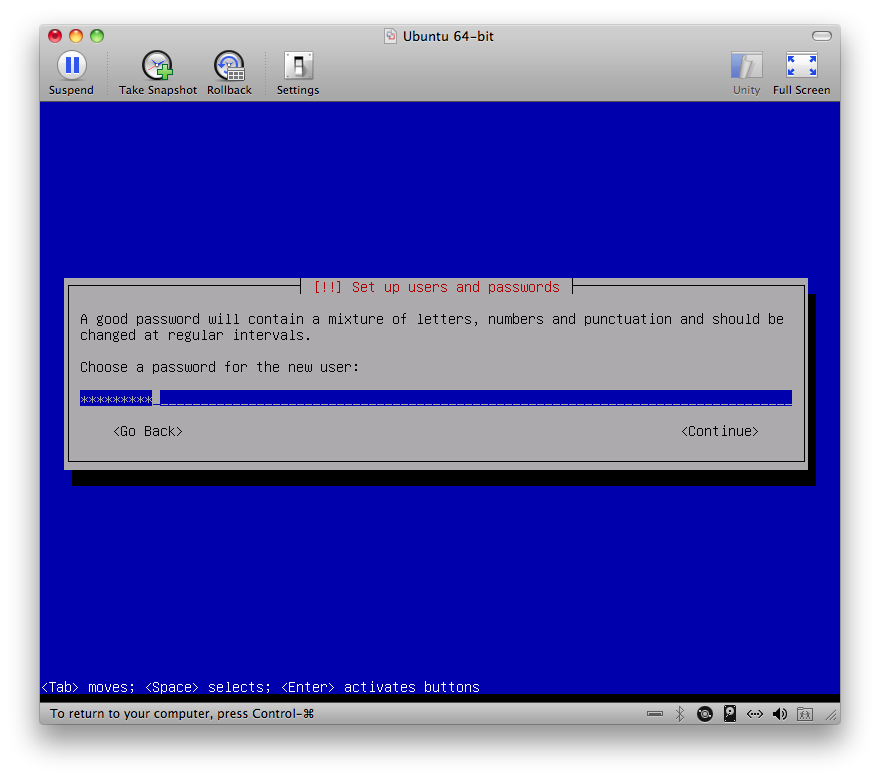
\includegraphics[width=0.75\textwidth]{screenshots/30_ubuntu_install.png}
\end{center}
\end{nofloat}
\newpage
Wir benötigen keinen HTTP-Proxy - daher einfach das Feld leer lassen
und mit der Eingabe-Taste bestätigen.

\begin{nofloat}{figure}
\begin{center}
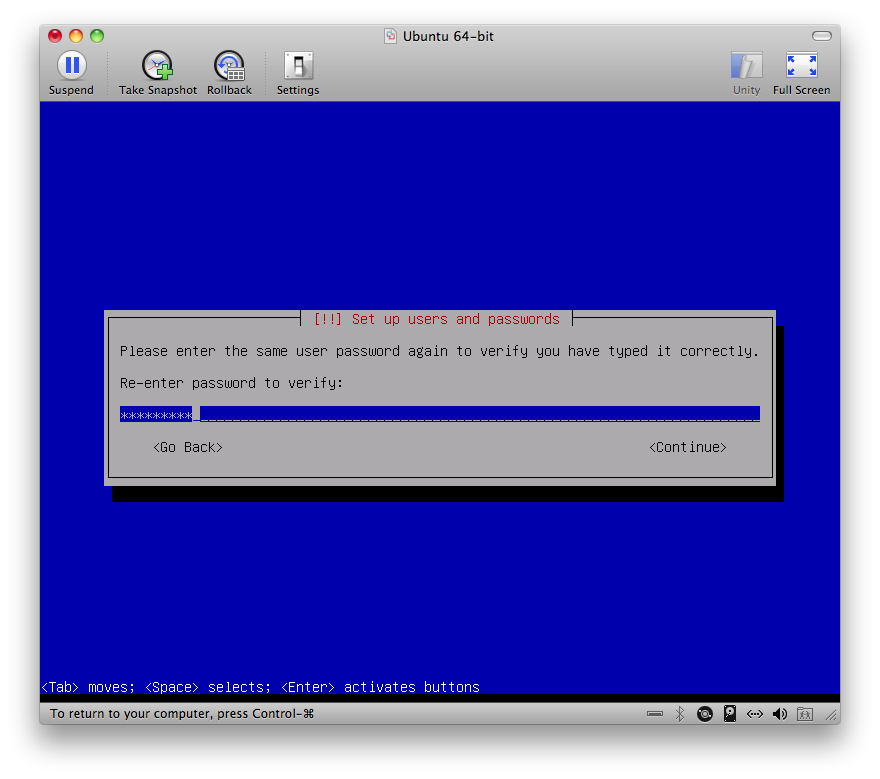
\includegraphics[width=0.75\textwidth]{screenshots/31_ubuntu_install.png}
\end{center}
\end{nofloat}

Wählen Sie hier \textbf{No automatic updates}.

\begin{nofloat}{figure}
\begin{center}
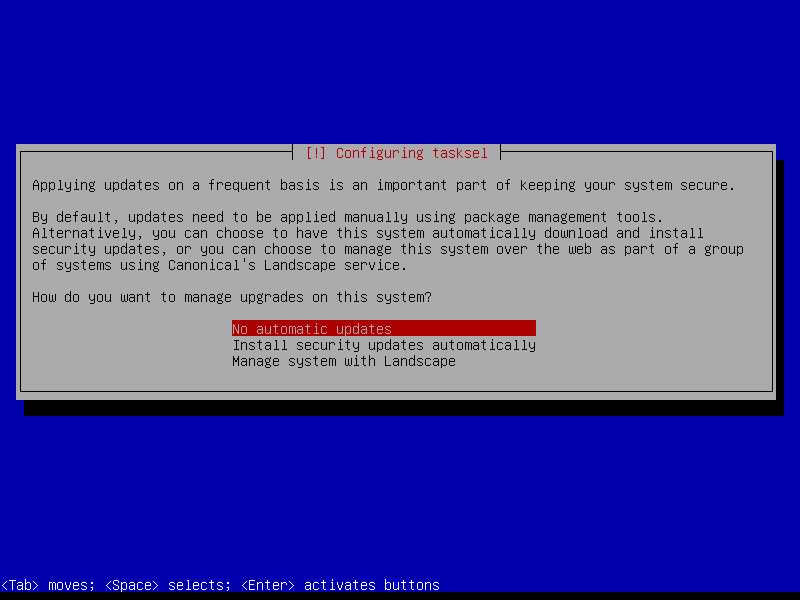
\includegraphics[width=0.75\textwidth]{screenshots/32_ubuntu_install.png}
\end{center}
\end{nofloat}
\newpage
Bei der zu installierenden Software wählen wir nur \textbf{OpenSSH server}.

\begin{nofloat}{figure}
\begin{center}
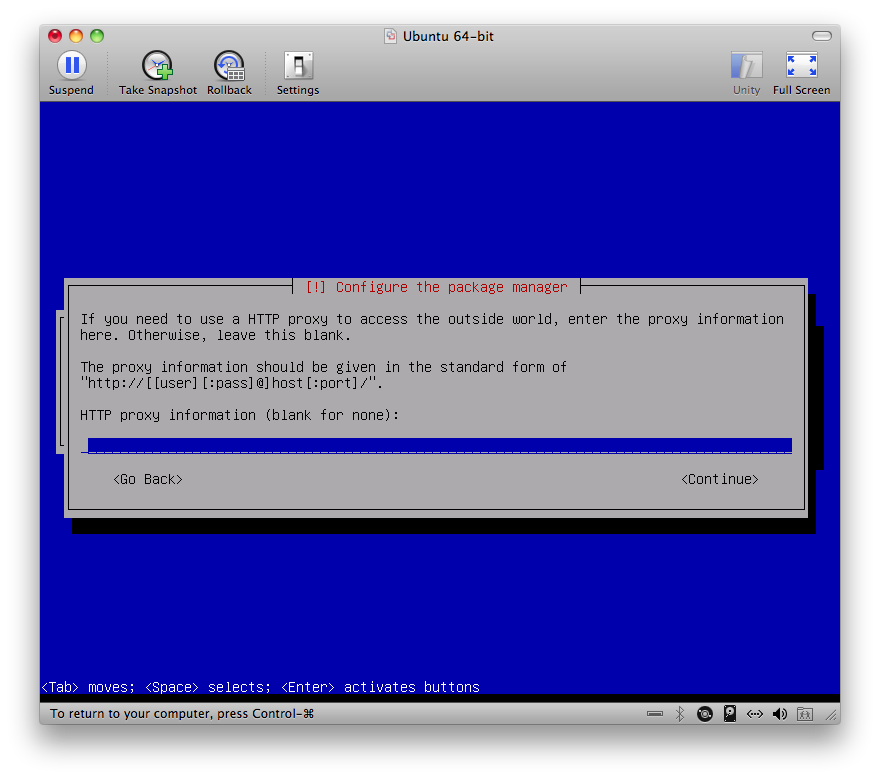
\includegraphics[width=0.75\textwidth]{screenshots/33_ubuntu_install.png}
\end{center}
\end{nofloat}

Nach der eigentlichen Installation wird nun der Bootloader GRUB installiert.
Wählen Sie hier \textbf{Yes}.

\begin{nofloat}{figure}
\begin{center}
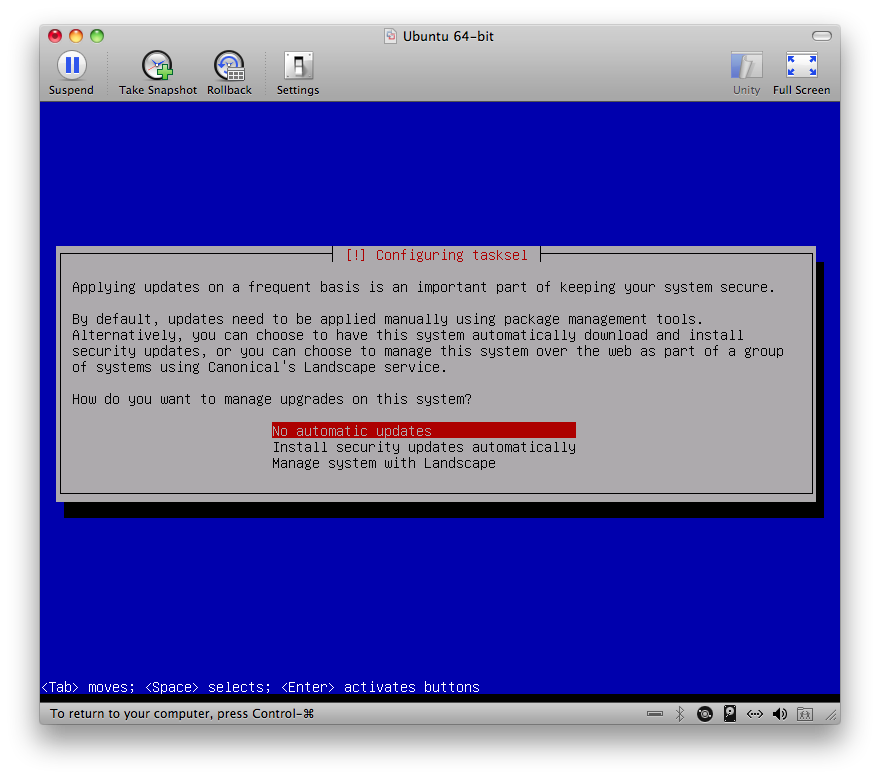
\includegraphics[width=0.75\textwidth]{screenshots/34_ubuntu_install.png}
\end{center}
\end{nofloat}
\newpage
Die Installation ist abgeschlossen. Hier einfach \textbf{Continue} wählen. Die
virtuelle Maschine startet nun neu und bootet das neu installierte System.

\begin{nofloat}{figure}
\begin{center}
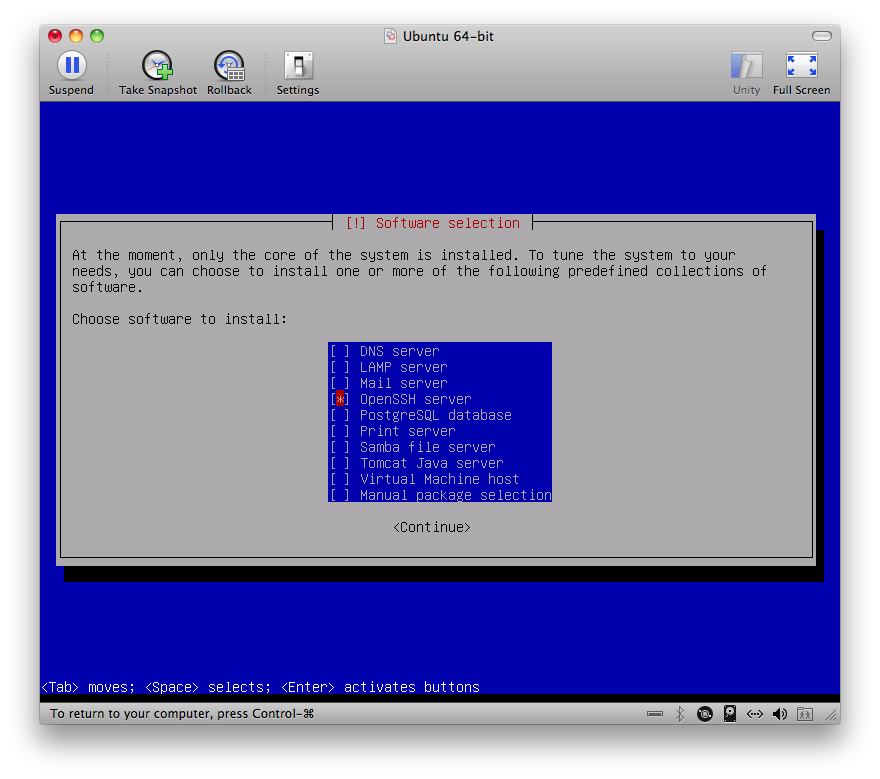
\includegraphics[width=0.75\textwidth]{screenshots/35_ubuntu_install.png}
\end{center}
\end{nofloat}

Verfahren Sie analog für den Server \textbf{srv201}.

%------------------------------------------------------------------------------
\subsection{Grundkonfiguration}
%------------------------------------------------------------------------------
Nach dem Neustart des virtuellen Servers kann man sich am System mit den zuvor
angelegten Benutzern angemeldet werden. Um das System zu abzusichern, ist eine
Anmeldung als Benutzer \textbf{root} nicht möglich. Um Administrationsaufgaben
durchführen zu können, kann der Benutzer \textbf{admin1} Kommandos unter einem
root-Kontext ausführen.

\begin{lstlisting}
sudo <command> [command parameter1] [command parameter2] 
\end{lstlisting}

Bei größeren Änderungen kann es hilfreich sein, eine root-Shell zu öffnen. Alle
Kommandos in dieser Shell werden unter root-Rechten ausgeführt, das Kommando
\textbf{sudo} ist dann nicht mehr notwendig. Die root-Shell kann mit 
\textbf{exit} beendet werden.

\begin{lstlisting}
sudo -s
\end{lstlisting}

Für die weitere Verwaltung ist es hilfreich das System zu aktualisieren.

\begin{lstlisting}
sudo aptitude update
sudo aptitude safe-upgrade 
\end{lstlisting}

Im Anschluss sind alle Programme aktualisiert. Für die weitere Einrichtung und
Fehlerdiagnose sind einige Programme und Tools hilfreich. Anbei eine kleine
Auswahl die bei der Durchführung des Versuches hilfreich sein können.
Als alternative Editoren zu \textbf{vi} können beispielsweise \textbf{nano}
oder \textbf{pico} installiert werden.

\begin{lstlisting}
sudo aptitude install vim tcpdump nmap
\end{lstlisting}

\textbf{Hinweis:} Falls bei der Installation der Servername falsch gesetzt
worden ist, kann dieser nachträglich in den folgenden Dateien geändert werden:
\begin{lstlisting}
sudo vi /etc/hostname
sudo vi /etc/hosts
\end{lstlisting}
Nach einem Neustart ist die Konfiguration vollständig übernommen.

%------------------------------------------------------------------------------
\subsection{Netzwerkkonfiguration}
%------------------------------------------------------------------------------
Für den Laboraufbau ist es notwendig, dass die Netzwerkkonfiguration vom
Benutzer vorgenommen wird:
\begin{lstlisting}
admin1@srv200$ sudo vi /etc/network/interfaces
\end{lstlisting}
Sie werden eventuell erneut zur Eingabe des Passwortes aufgefordert. Die Datei
sollte danach folgenden Inhalt haben:
\begin{scriptsize}
\begin{lstlisting}
# This file describes the network interfaces available on your system
# and how to activate them. For more information, see interfaces(5).

# The loopback network interface
auto lo
iface lo inet loopback

# The primary network interface
auto eth0
iface eth0 inet static
  address 10.174.26.200
  netmask 255.255.255.0
  gateway 10.174.26.254
  network 10.174.26.0
  broadcast 10.174.26.255
\end{lstlisting}
\end{scriptsize}

Jetzt sollte noch die Konfiguration der Namensauflösung angepasst werden:
\begin{lstlisting}
admin1@srv200$ sudo vi /etc/resolv.conf
\end{lstlisting}
Diese Datei sollte danach folgenden Inhalt haben:
\begin{scriptsize}
\begin{lstlisting}
nameserver 10.174.26.126
domain beta.tklabor.site
search beta.tklabor.site
\end{lstlisting}
\end{scriptsize}
Starten Sie anschließend das System neu:
\begin{lstlisting}
admin1@srv200$ sudo reboot
\end{lstlisting}
Verfahren Sie analog für den Server \textbf{srv201}.

%------------------------------------------------------------------------------
\subsection{Funktionstest}
%------------------------------------------------------------------------------
Bevor die Installation der Serverdienste erfolgt, testen Sie die Konfiguration:
\begin{enumerate}
  \item Layer-3 Konnektivität zwischen den beiden Servern srv200 und srv201
  \item Lokale Namensauflösung auf srv200 für den hostnamen
  \textbf{srv200.beta.tklabor.site}.
  \item Layer-3 Konnektivität auf den zentralen Router für den Internetzugang
  \item Namensauflösung ins Internet und Layer-3 Konnektivität ins Internet
  \item Führen Sie die Tests analog auf srv201 durch.
\end{enumerate}

Sind alle Tests erfolgreich, können Sie mit der weiteren Konfiguration
fortfahren.
